\documentclass[cn,10pt]{elegantbook}

\title{Linux云计算}
\subtitle{课程学习笔记}

\author{雨霓同学}
\institute{Azurekite}
\date{May 2, 2021}
\version{2.1}
\bioinfo{邮箱}{sx12101184@qq.com}

\extrainfo{在没有结束前,总要做很多没有意义的事,这样才可以在未来某一天,用这些无意义的事去堵住那些讨厌的缺口。}

\setcounter{tocdepth}{3}
\usepackage{minted}
\logo{233.png}
\cover{sd12s.png}
\usepackage{longtable}
\usepackage{easyphys}
\usepackage{wrapfig}
\newcommand{\ccr}[1]{\makecell{{\color{#1}\rule{1cm}{1cm}}}}

\definecolor{customcolor}{RGB}{245, 255, 250}
\colorlet{coverlinecolor}{customcolor}

\usepackage{fontawesome}
\usepackage[many]{tcolorbox}
\usetikzlibrary{arrows,positioning,calc,fadings,shapes,decorations.markings}
\usepackage{circuitikz}
\usepackage{float}
\definecolor{lsp}{RGB}{0,174,247}
\usepackage{tikz}
\usepackage{mathtools}
\usepackage{mdframed}
\BeforeBeginEnvironment{minted}{\begin{mdframed}[backgroundcolor=gray!5,hidealllines=true,innerrightmargin=0pt,linecolor=gray!70,skipabove=2pt,everyline=true,leftmargin=3mm,innerbottommargin=0pt]}
\AfterEndEnvironment{minted}{\end{mdframed}}
\usetikzlibrary{backgrounds,calc,shadows}
\usepackage[object=vectorian]{pgfornament} %% 
\usepackage{fontspec}
\setmonofont{CMU Typewriter Text}
\usepackage{xcolor}
\tcbuselibrary{minted}
\tcbuselibrary{listings}
\definecolor{mlblue3}{RGB}{44, 49, 51} % mycmd颜色
\definecolor{mlblue2}{RGB}{35, 41, 55}
\definecolor{bg}{rgb}{0.99,0.99,0.99}
\definecolor{Green}{rgb}{199, 231, 228}
\definecolor{mlblue}{RGB}{236,243,255}
\definecolor{mblue}{RGB}{0,123,255}
\newcommand{\md}[1]{{\color{purple}#1}}
\newcommand{\keypoint}[1]{\textbf{\textcolor{red}{#1}}}
\newcommand{\cmt}{\noindent\hspace{-0.25em}\textcolor{Green}{\ding{226}} \hspace{0.2em}}
\newcommand{\sol}{\noindent\hspace{-0.12em}\textcolor{cyan}{\ding{45}} \hspace{0.2em}}
\newcommand{\solc}{\noindent\hspace{-0.12em}\textcolor{cyan}{\ding{45}} \hspace{0.2em} \vspace*{-\baselineskip}}
\definecolor{mlred}{RGB}{253,243,242}
\definecolor{mred}{RGB}{220,53,69}
% highlight environment
\newenvironment{ilight}
{\centering
	\vspace*{6pt}
	\begin{tcolorbox}[colframe=Gray,colback=LightGrey!15]
		\setlength{\baselineskip}{\baselineskip}%
	}
	{\end{tcolorbox}\vspace*{-4pt}}

%%%%%%%%%%%%%%%%%%%%%%%%%%%%%%%
%mycmd定制
%%%%%%%%%%%%%%%%%%%%%%%%%%%%%%%
\newtcblisting{mycmd}[2]{colback=black,
	colupper=white,
	colback=mlblue3,
	frame style={opacity=0.25},
	colframe=mlblue3,
	center title,
	left = 2pt,
	width=\linewidth,
	listing only,
	drop shadow,
	right = 2pt,
	top = 2mm,
	boxsep =2pt,
	arc=2pt,
	fonttitle=\small\ttfamily\bfseries,
	title ={\faCode \hspace*{\fill} #1 \hspace*{\fill}\faRemove\\
		文件(F)\quad 动作(A)\quad 编辑(E)\quad 查看(V)\quad 帮助(H)\hspace*{\fill}},
	listing options={style=tcblatex,language=sh},
	every listing line={\textcolor{red}{\small\ttfamily\bfseries #2 \$> }}
}

%%%%%%%%%%%%%%%%%%%%%%%%%%%%%%%
%mycmd2定制
%%%%%%%%%%%%%%%%%%%%%%%%%%%%%%%
\newtcolorbox{mycmd2}[1]{colback=black,
	colupper=white,
	colback=mlblue3,
	frame style={opacity=0.25},
	colframe=mlblue3,
	center title,
	left = 2pt,
	width=\linewidth,
	listing only,
	drop shadow,
	right = 2pt,
	top = 1mm,
	boxsep =1pt,
	arc=2pt,
	fonttitle=\small\ttfamily\bfseries,
	title ={\faCode \hspace*{\fill} #1 \hspace*{\fill}\faRemove\\文件(F)\quad 动作(A)\quad 编辑(E)\quad 查看(V)\quad 帮助(H)\hspace*{\fill}},
	listing options={style=tcblatex,language=sh},}

\lstdefinestyle{HTML}{
	language =  bash, % 语言选Python
	frame=none,
	mathescape,
	basicstyle = {\small\ttfamily\bfseries\color{white}},
	emphstyle={ \small\ttfamily\bfseries\color{red}},
	numbers=none,
	stepnumber=2,
	numbersep=3em,
	numberstyle= \small\ttfamily\bfseries,
	keywordstyle    = \small\ttfamily\bfseries\color{red!60},
	stringstyle     =   \small\ttfamily\bfseries\color{white},
	breaklines      =   true,   % 自动换行,
	columns         =   fixed,  %字间距就不固定很丑,必须加
	basewidth       =  .5em,
	commentstyle=\small\ttfamily\bfseries\color{white},
	backgroundcolor=\color[RGB]{44, 49, 51},
	tabsize=4,
	showspaces=false,
	showstringspaces=false,
	morekeywords={ls,cd},
}
\lstdefinestyle{text}{
	language =   HTML, % 语言选Python
	frame=topline,
	mathescape,
	emphstyle={\color{frenchplum}},
	numbers=none,
	stepnumber=2,
	numbersep=3em,
	numberstyle=\tiny,
	rulecolor = \color{black},
	keywordstyle    =   \color{blue},
	stringstyle     =   \color{magenta},
	commentstyle    =   \color{red},
	breaklines      =   true,   % 自动换行,
	columns         =   fixed,  %字间距就不固定很丑,必须加
	basewidth       =   .5em,
	keywordstyle=\color{red},
	commentstyle=\color{gray},
	backgroundcolor=\color[RGB]{218, 218, 218},
	tabsize=4,
	showspaces=false,
	showstringspaces=false,
	columns=fixed,
	morekeywords={maketitle,pip,matplotlib,pandas,numpy,np,dtype,In [],Out []},
}
%%%%%%%%%%%%%%%%%%%%%%%%%%%%%%%%%
\newfontfamily\bfont{Source Code Pro}
\newminted{vim}{gobble=2,linenos}

\setminted[vim]{breaklines,
breakanywhere,
escapeinside=||,
highlightcolor=orange!10,
linenos=true,
framesep=3pt,
frame=bottomline,
framerule=2pt,
rulecolor=\color{black!35},
style=colorful,
breaklines=true,
}
\setminted[nginx]{breaklines,
breakanywhere,
escapeinside=||,
highlightcolor=green!30,
linenos=true,
framesep=3pt,
frame=bottomline,
framerule=2pt,
rulecolor=\color{black!35},
style=colorful,
breaklines=true,
}

\setminted[shell]{breaklines,
linenos=true,
bgcolor=blue!10,
breakautoindent=false,
breaksymbolleft=\raisebox{0.8ex}{
\small\reflectbox{\carriagereturn}},
breaksymbolindentleft=0pt,
frame=bottomline,
framesep=1pt,
framerule=1pt,
rulecolor=\color{black!35},
breaksymbolsepleft=0pt,
breaksymbolright=\small\carriagereturn,
breaksymbolindentright=0pt,
}
\lstdefinestyle{linux}{
	language = sh , % 语言选Python
	frame=b,
	aboveskip=3mm,
	belowskip=3mm,
	showstringspaces=false,
	columns=flexible,
	framerule=1pt,
	rulecolor=\color{black!35},
	backgroundcolor=\color{gray!5},
	basicstyle={\small\ttfamily},
	numbers=left,
	numberstyle=\tiny\color{black},
	comment=[is]{!/*}
	commentstyle=\color{green!60},
	stringstyle=\color{blue},
	breaklines=true,
	breakatwhitespace=true,
	tabsize=3,
	morekeywords={bind-utils,}
	classoffset=0,
	morekeywords={root@localhost,},keywordstyle=\color{orange},
	classoffset=1,
	morekeywords={yum,bind-utils},keywordstyle=\color{blue},
	classoffset=0,
}

\lstdefinestyle{linux2}{
	language =  bash , % 语言选Python
	frame=none,
%	aboveskip=4mm,
%	belowskip=4mm,
	showstringspaces=false,
	framesep=1pt,
	columns=flexible,
	framerule=2pt,
	aboveskip=1em,
	numbersep=12pt,
	rulecolor=\color{black},
	backgroundcolor=\color{gray!5},
	basicstyle={\small\bfont},
	numbers=left,
	numberstyle=\tiny\color{black!80},
	keywordstyle=\color{blue},
	comment=[is]{!/*}
	commentstyle=\color{green!60},
	stringstyle=\color{blue},
	breaklines=true,
	breakatwhitespace=true,
	tabsize=3,
	morekeywords={ls,mkdir,-,|},
}

\lstdefinestyle{python}{
	language =   python, % 语言选Python
	frame=b,
	mathescape,
	emphstyle={\small\ttfamily\bfseries\color{frenchplum}},
	numbers=left,
	stepnumber=1,
	numbersep=3em,
	numberstyle= \small\ttfamily\bfseries\tiny,
	keywordstyle    =  \small\ttfamily\bfseries\color{orange},
	stringstyle     =  \small\ttfamily\bfseries\color{red},
	breaklines      =   true,   % 自动换行,
	columns         =   fixed,  %字间距就不固定很丑,必须加
	basewidth       =   .5em,
	commentstyle=\small\ttfamily\bfseries\color{cyan},
	backgroundcolor=\color[RGB]{250, 250, 250},
	tabsize=4,
	showspaces=false,
	showstringspaces=false,
	morekeywords={},
}
\lstdefinestyle{python2}{
	language =   Python, % 语言选Python
	frame=none,
	basicstyle={\small\ttfamily\bfseries\color{white}},
	mathescape,
	emphstyle={\small\ttfamily\bfseries\color{white}},
	numbers=none,
	stepnumber=2,
	numbersep=3em,
	numberstyle= \small\ttfamily\bfseries\tiny,
	keywordstyle    =  \small\ttfamily\bfseries\color{orange},
	stringstyle     =  \small\ttfamily\bfseries\color{white},
	breaklines      =   true,   % 自动换行,
	columns         =   fixed,  %字间距就不固定很丑,必须加
	basewidth       =   .5em,
	commentstyle=\small\ttfamily\bfseries\color{cyan!30},
	backgroundcolor=\color{mlblue3},
	tabsize=4,
	showspaces=false,
	showstringspaces=false,
	morekeywords={Out,In,maketitle,pip,matplotlib,pandas,numpy,np,dtype},
}
\lstdefinestyle{python3}{
	language =   Python, % 语言选Python
	frame=none,
	basicstyle={\small\ttfamily\bfseries\color{white}},
	mathescape,
	emphstyle={\small\ttfamily\bfseries\color{white}},
	numbers=none,
	stepnumber=2,
	numbersep=3em,
	numberstyle= \small\ttfamily\bfseries\tiny,
	keywordstyle    =  \small\ttfamily\bfseries\color{orange},
	stringstyle     =  \small\ttfamily\bfseries\color{white},
	breaklines      =   true,   % 自动换行,
	columns         =   fixed,  %字间距就不固定很丑,必须加
	basewidth       =   .5em,
	commentstyle=\small\ttfamily\bfseries\color{cyan!30},
	backgroundcolor=\color{macosbox@bgdark},
	tabsize=4,
	showspaces=false,
	showstringspaces=false,
	morekeywords={Out,In,maketitle,pip,matplotlib,pandas,numpy,np,dtype},
}
\lstdefinestyle{python4}{
	language =   Python, % 语言选Python
	frame=none,
	mathescape,
	emphstyle={\small\ttfamily\bfseries\color{frenchplum}},
	numbers=none,
	stepnumber=2,
	numbersep=3em,
	numberstyle= \small\ttfamily\bfseries\tiny,
	keywordstyle    =  \small\ttfamily\bfseries\color{orange},
	stringstyle     =  \small\ttfamily\bfseries\color{magenta},
	breaklines      =   true,   % 自动换行,
	columns         =   fixed,  %字间距就不固定很丑,必须加
	basewidth       =   .5em,
	commentstyle=\small\ttfamily\bfseries\color{cyan},
	backgroundcolor=\color{macosbox@bg},
	tabsize=4,
	showspaces=false,
	showstringspaces=false,
	morekeywords={Out,In,maketitle,pip,matplotlib,pandas,numpy,np,dtype},
}
%%%%%%%%%%%%%%%%%%%%%%%
\newtcolorbox{code}[1][]{%
	enhanced jigsaw,
	breakable,
	borderline west={1.5pt}{0pt}{mblue},
	sharp corners,
	boxrule=0pt,
	fonttitle={\small\ttfamily\bfseries},
	coltitle={black},
	title={{\color{mblue} \faCode} \quad Python Code:\ },
	colbacktitle=mlblue,
	colback=bg,
	left=2mm,
	right=2mm,
	#1}
%%%%%%%%%%%%%%%%%%%%%%%%%%%%%
\tcbset{
	myexample/.style={
		enhanced,
		width=\linewidth,
		colback=white, % 背景颜色 red!5!white
		colframe=gray!20, % 外框的颜色
		fonttitle=\bfseries,
		breakable,
		arc=2pt,
		drop shadow={gray!15,opacity=1},
		titlerule=0pt,
		title style={fill=white},
		coltitle=gray,
		drop shadow,
		highlight math style={reset,colback=white,colframe=black}
	}
}
\newtcolorbox{sBox}{myexample}
%%%%%%%%%%%%%%%%%%%%%%%%%%%%%%%%%%%%%%%%%
\newtcolorbox{notes}[1][]{%
	enhanced jigsaw,
	borderline west={1.5pt}{0pt}{mblue},
	sharp corners,
	boxrule=0pt,
	fonttitle={\small\bfseries},
	coltitle={black},
	title={{\color{mblue} \faInfoCircle} Note:\ },
	colbacktitle=mlblue,
	colback=bg,
	left=2mm,
	right=2mm,
	#1}

%%%%%%%%%%%%%%%%%%%%%%%%%%%
\newtcolorbox{warning}[1][]{%
	enhanced jigsaw,
	breakable,
	borderline west={1.5pt}{0pt}{mred},
	sharp corners,
	boxrule=0pt,
	fonttitle={\small\bfseries},
	coltitle={black},
	title={{\color{mred} \faExclamationTriangle} Warning:\ },
	colbacktitle=mlred,
	colback=bg,
	left=2mm,
	right=2mm,
	#1}
%%%%%%%%%%%%%%%%%%%%%%%%%%%%%
\newenvironment{macosbox}[2][]{
	\begin{tcolorbox}[enhanced,
		coltitle=black,
		colback=macosbox@bg,
		boxrule=0mm,
		frame style={draw=macosbox@bord,fill=macosbox@bord},
		title style={top color=macosbox@top,bottom color=macosbox@bot},
		drop fuzzy shadow=black,
		#1, %hbox
		title=\hspace*{-3mm}%
		\macosbox@dot{macosbox@red} %
		\macosbox@dot{macosbox@yellow} %
		\macosbox@dot{macosbox@green}%
		\hspace*{\fill}\hspace*{-10mm}#2\hspace*{\fill}]
		\ifthenelse{\isundefined{\usemintedstyle}}{}{\usemintedstyle{\macosbox@mintedstyle}}
		\color{macosbox@textcol}
	}{
	\end{tcolorbox}
}
%%%%%%%%%%%%%%%%%%%%%%%%%%%%%%%%%%%%%%%%%%%%%%%%%%%%%%%%%%%%%%
\newtcolorbox{macbox}[2][]{%
	enhanced,
	coltitle=black,
	colback=macosbox@bg,
	boxrule=0mm,
	frame style={draw=macosbox@bord,fill=macosbox@bord},
	title style={top color=macosbox@top,bottom color=macosbox@bot},
	drop fuzzy shadow=black,
	title={{\textcolor[RGB]{236, 96, 92}{\faCircle}
			\textcolor[RGB]{247, 188, 44}{\faCircle}
			\textcolor[RGB]{88, 204, 65}{\faCircle}
			\hspace*{\fill}\hspace*{-10mm}\texttt{#2}\hspace*{\fill}}},#1
}
\newtcolorbox{macboxd}[2][]{%
	enhanced,
	colupper=white,
	coltitle=white,
	colback=macosbox@bgdark,
	boxrule=0mm,
	frame style={draw=macosbox@borddark,fill=macosbox@borddark},
	title style={top color=macosbox@topdark,bottom color=macosbox@botdark},
	drop fuzzy shadow=black,
	title={{\textcolor[RGB]{236, 96, 92}{\faCircle}
			\textcolor[RGB]{247, 188, 44}{\faCircle}
			\textcolor[RGB]{88, 204, 65}{\faCircle}\hspace*{\fill}\hspace*{-10mm}\texttt{#2}\hspace*{\fill}}},
	#1
}
%%%%%%%%%%%%%%%%%%%%%%%%%%%%%
\definecolor{macosbox@red}{RGB}{236,96,92}
\definecolor{macosbox@yellow}{RGB}{247,188,44}
\definecolor{macosbox@green}{RGB}{88,204,65}

\definecolor{macosbox@top}{RGB}{237,237,237}
\definecolor{macosbox@bot}{RGB}{189,189,189}
\definecolor{macosbox@bord}{RGB}{182,176,176}
\definecolor{macosbox@bg}{RGB}{240,240,240}
\definecolor{macosbox@textcol}{RGB}{50,50,50}

\definecolor{macosbox@topdark}{RGB}{96,96,98}
\definecolor{macosbox@botdark}{RGB}{44,45,47}
\definecolor{macosbox@borddark}{RGB}{13,13,15}
\definecolor{macosbox@bgdark}{RGB}{55,56,58}
\definecolor{macosbox@textcoldark}{RGB}{223,224,226}

\lstdefinestyle{text}{
	language =   HTML, % 语言选Python
	frame=topline,
	mathescape,
	emphstyle={\color{frenchplum}},
	numbers=none,
	stepnumber=2,
	numbersep=3em,
	numberstyle=\tiny,
	rulecolor = \color{black},
	keywordstyle    =   \color{blue},
	stringstyle     =   \color{magenta},
	commentstyle    =   \color{red},
	breaklines      =   true,   % 自动换行,
	columns         =   fixed,  %字间距就不固定很丑,必须加
	basewidth       =   .5em,
	keywordstyle=\color{red},
	commentstyle=\color{gray},
	backgroundcolor=\color[RGB]{218, 218, 218},
	tabsize=4,
	showspaces=false,
	showstringspaces=false,
	columns=fixed,
	morekeywords={maketitle,pip,matplotlib,pandas,numpy,np,dtype,In [],Out []},
}



\usepackage{minitoc}
\usepackage{wallpaper}
\definecolor{ocre}{RGB}{146, 218, 243}
\makeatletter
\newcommand{\@mypartnumtocformat}[2]{%
	\setlength\fboxsep{0pt}%
	\noindent\colorbox{orange!60}{\strut\parbox[c][.7cm]{\ecart}{\color{ocre!70}\Large\sffamily\bfseries\centering#1}}\hskip\esp\colorbox{ocre!40}{\strut\parbox[c][.7cm]{\linewidth+0.2cm-\ecart-\esp}{\partname\Large\sffamily\centering 第#1部分 * #2}}}%
%%%%%%%%%%%%%%%%%%%%%%%%%%%%%%%%%%
% unnumbered part in the table of contents
\newcommand{\@myparttocformat}[1]{%
	\setlength\fboxsep{0pt}%
	\noindent\colorbox{ocre!40}{\strut\parbox[c][.7cm]{\linewidth}{\Large\sffamily\centering#1}}}%
%%%%%%%%%%%%%%%%%%%%%%%%%%%%%%%%%%
\newlength\esp
\setlength\esp{4pt}
\newlength\ecart
\setlength\ecart{1.2cm-\esp}
\newcommand{\thepartimage}{}%
\newcommand{\partimage}[1]{\renewcommand{\thepartimage}{#1}}%

%----------------------------------------------------------------------------------------
%	MINI TABLE OF CONTENTS IN PART HEADS
%----------------------------------------------------------------------------------------

% Chapter text styling

\newcommand{\thepartimages}{}%
\newcommand{\partimages}[1]{\ifusepartimage\renewcommand{\thepartimages}{#1}\fi}%
\def\@part[#1]#2{%
	\ifnum \c@secnumdepth >-2\relax
	\refstepcounter{part}%
	\addcontentsline{toc}{part}{\texorpdfstring{\protect\@mypartnumtocformat{\arabic{part}}{#1}}{\partname~\thepart\ ---\ #1}}
	\else
	\addcontentsline{toc}{part}{\texorpdfstring{\protect\@myparttocformat{#1}}{#1}}%
	\fi
	\markboth{}{}%
	{\ThisCenterWallPaper{1.1}{12.png}
		\centering
		\vspace{-6cm}
		\interlinepenalty \@M
		\normalfont
		\ifnum \c@secnumdepth >-2\relax
		\huge\bfseries \partname  \thepart  * 
%		\vskip 20\p@
		\fi
		\huge \bfseries #2\par
		\hbox{%
	\vbox{%
		\vspace{-4cm}
		\hsize=7mm%
		\begin{tabular}{@{}p{7mm}@{}}
			\makebox[7mm]{\scshape\strut\small}\\
			\makebox[7mm]{\cellcolor{black}\Huge\color{white}\bfseries\strut\rule[-4cm]{0pt}{4cm}}%
		\end{tabular}%
		\makebox(0,0){\put(-10,-100){\fbox{\phantom{\rule[-4cm]{7mm}{4cm}}}}}
	}%
	\kern-2pt
	\vbox to 0pt{%
		\tabular[t]{@{}p{1cm}p{\dimexpr\hsize-2.1cm}@{}}\hline
		& \Huge\itshape\rule{0pt}{1.5\ht\strutbox}\endtabular}}%	
}%
	\@endpart}
\def\@spart#1{%
	{\centering
		\interlinepenalty \@M
		\normalfont
		\Huge \bfseries #1\par}%
	\@endpart}
\def\@endpart{\vfil\newpage
	\if@twoside
	\if@openright
	\null
	\thispagestyle{empty}%
	\newpage
	\fi
	\fi
	\if@tempswa
	\twocolumn
	\fi}

%----------------------------------------------------------------------------------------
%	CHAPTER HEADINGS
%----------------------------------------------------------------------------------------

% A switch to conditionally include a picture, implemented by Christian Hupfer
\newif\ifusechapterimage
\usechapterimagetrue
\newcommand{\thechapterimage}{}%
\newcommand{\chapterimage}[1]{\ifusechapterimage\renewcommand{\thechapterimage}{#1}\fi}%
\newcommand{\autodot}{{\color{structurecolor}\faModx}}
\def\@makechapterhead#1{%
	{\parindent \z@ \raggedright \normalfont
		\ifnum \c@secnumdepth >\m@ne
		\if@mainmatter
		\begin{tikzpicture}[remember picture,overlay]
			\node at (current page.north west)
			{\begin{tikzpicture}[remember picture,overlay]
					\node[anchor=north west,inner sep=0pt] at (0,0) {\ifusechapterimage\includegraphics[width=\paperwidth]{\thechapterimage}\fi};
					\draw[anchor=west] (\Gm@lmargin+3.3cm,-9cm) node [line width=2pt,rounded corners=15pt,draw=ocre,fill=white,fill opacity=0.5,inner sep=15pt]{\strut\makebox[22cm]{}};
					\draw[anchor=west] (\Gm@lmargin+3.9cm,-9cm) node {\huge\kaishu\bfseries\color{black} 第 \thechapter 章  \autodot\color{black}~#1\strut};
			\end{tikzpicture}};
		\end{tikzpicture}
		\else
		\begin{tikzpicture}[remember picture,overlay]
			\node at (current page.north west)
			{\begin{tikzpicture}[remember picture,overlay]
					\node[anchor=north west,inner sep=0pt] at (0,0) {\ifusechapterimage\includegraphics[width=\paperwidth]{\thechapterimage}\fi};
					\draw[anchor=west] (\Gm@lmargin+3.3cm,-9cm) node [line width=2pt,rounded corners=15pt,draw=ocre,fill=white,fill opacity=0.5,inner sep=15pt]{\strut\makebox[22cm]{}};
					\draw[anchor=west] (\Gm@lmargin+3.9cm,-9cm) node {\huge\sffamily\bfseries\color{black}#1\strut};
			\end{tikzpicture}};
		\end{tikzpicture}
		\fi\fi\par\vspace*{270\p@}}}

%-------------------------------------------

\def\@makeschapterhead#1{%
	\begin{tikzpicture}[remember picture,overlay]
		\node at (current page.north west)
		{\begin{tikzpicture}[remember picture,overlay]
				\node[anchor=north west,inner sep=0pt] at (0,0) {\ifusechapterimage\includegraphics[width=\paperwidth]{\thechapterimage}\fi};
				\draw[anchor=west] (\Gm@lmargin+3.3cm,-9cm) node [line width=2pt,rounded corners=15pt,draw=ocre,fill=white,fill opacity=0.5,inner sep=15pt]{\strut\makebox[22cm]{}};
				\draw[anchor=west] (\Gm@lmargin+3.9cm,-9cm) node {\huge\sffamily\bfseries\color{black}#1\strut};
		\end{tikzpicture}};
	\end{tikzpicture}
	\par\vspace*{270\p@}}

\pagenumbering{arabic}

\usepackage{titletoc} % Required for manipulating the table of contents

\contentsmargin{0cm} % Removes the default margin
\setcounter{secnumdepth}{5}
% Part text styling (this is mostly taken care of in the PART HEADINGS section of this file)
\titlecontents{part}
[0cm] % Left indentation
{\addvspace{20pt}\bfseries} % Spacing and font options for parts
{}
{}
{}

\titlecontents{chapter}
[16mm] % Left indentation
{\bfseries} % Spacing and font options for parts
{\contentslabel[\heiti 第~\thecontentslabel 章]{16mm}}
{}
%{[0.5pc]{$\cdot$}\contentspage[{\makebox[0pt][r]{\thecontentspage}}]}
{\titlerule*[0.5pc]{~ }\contentspage}
\makeatother

\usepackage{graphicx}
\usepackage{xhfill}
\newcommand{\fancyline}[2][\ding{36}]{\noindent\ #1\xdotfill{1pt}[ocre]#1\xdotfill{1pt}[ocre]#1\
}

%%%%%%%%%%%%%%%%%%%%%%%%%%%%%%%%%%%%%%%%
\usepackage{ifthen}
\usetikzlibrary{shadows}
\usepackage{afterpage}
\newcommand\myemptypage{
	\null
	\thispagestyle{empty}
	\addtocounter{page}{-1}
	\newpage
}
\usepackage{booktabs,colortbl}
\colorlet{tableheadcolor}{gray!25} % Table header colour = 25% gray
\newcommand{\headcol}{\rowcolor{tableheadcolor}} %
\newcommand{\hdrule}[1]{\begin{ascolorbox101}{#1}\end{ascolorbox101}}
\newcommand{\btrule}[1]{\begin{ascolorbox102}{#1}\end{ascolorbox102}}
\begin{document}

\maketitle

\myemptypage

\frontmatter
\begin{center}
	\textbf{\LARGE 模板概述}
\end{center}
\begin{ascolorbox5}{模板参考使用说明}
本模板主要参考了以下几个模板,在Elegant\LaTeX{} 系列模板的模板上,参考使用了The Legrand Orange Book模板众的章节设计,最后参考使用了A-Level-Physics模板当中很多tcolorbox环境.
\begin{ascboxB}{Elegant\LaTeX{} 系列模板}
ElegantLATEX 项目组致力于打造一系列美观、优雅、简便的模板方便用户使用。目前由
ElegantNote,ElegantBook,ElegantPaper 组成,分别用于排版笔记,书籍和工作论文。
\begin{itemize}
	\item 官网:\href{https://elegantlatex.org/}{https://elegantlatex.org/}
	\item GitHub 网址:\href{https://github.com/ElegantLaTeX/}{https://github.com/ElegantLaTeX/}
\end{itemize} 
\end{ascboxB}
\begin{ascboxB}{The Legrand Orange Book}
这本书模板具有优雅的布局,带有漂亮的标题页和部分/章节标题。该模板最初由Mathias Legrand创作,灵感来自此处和此处的材料。
\begin{itemize}
\item  模板地址:\href{http://www.latextemplates.com/template/the-legrand-orange-book}{http://www.latextemplates.com/template/the-legrand-orange-book}
\item  latexstudio网站下载网址:\href{https://www.latexstudio.net/index/details/index/mid/264}{https://www.latexstudio.net/index/details/index/mid/264}
\item 本文主要参考了该模板的章节图设计以及目录设计属于,比较遗憾的是章节部分的小目录未实现
\end{itemize} 
\end{ascboxB}
\begin{ascboxB}{A-Level-Physics}
本书原来模板源于原作者 \keypoint{colin-young} \url{colin-young@live.com},因计划用于教师教材用书,故在其中设置了诸多的 tcolorbox 环境,并整理于:\url{https://marukunalufd0123.hatenablog.com/entry/2019/03/15/071717}.模板设置了大量的tcolorbox环境,适用于课前知识预习、知识点标题、段文关键词、练习,习题,解答、思考,知识回顾,延伸与探究等诸多环境。
\begin{itemize}
	\item 模板下载地址:\href{https://www.latexstudio.net/index/details/index/mid/1269}{https://www.latexstudio.net/index/details/index/mid/1269}
	\item 本文参考了其中大部分的tcolorbox环境设计
\end{itemize} 	
\end{ascboxB}

\md{在此特别感谢legant\LaTeX{} 系列模板,The Legrand Orange Book模板,A-Level-Physics模板的各位作者}
\end{ascolorbox5}
\begin{flushright}
	Azurekite \& 雨霓同学 \& 1210 \\
	2022/01/03 21:35:10
\end{flushright}
{\large
	\noindent {\color{red} 在此感谢为本书做出贡献的成员}   雨霓同学\\
}
\begin{sBox}
	\begin{center}
		\noindent\footnotesize\begin{tabular}{@{}l@{ }l|l@{ }l@{}}
			\textcolor[RGB]{18,183,245}{\faQq}:&910014191:  这是QQ!一起搞事情!\faSendO   & \textcolor[RGB]{9,187,7}{\faWeixin}:&\verb|雨霓同学|  公众号,知识与资源分享[没有运营]\faSendO \\
			\textcolor[RGB]{0,194,255}{\faInternetExplorer}:& \href{https://www.cnblogs.com/1210x1184/}{ 博客园},技术分享  & {\textcolor[RGB]{39,165,188}{\faGithubAlt}}:& \href{https://github.com/Azure1210/}{Github}  什么都没写,先放这里了 \\
			\textcolor[RGB]{18,183,245}{\faWeibo}\textbf{:} & \href{https://weibo.com/u/5713129191}{微博} \faSendO 多多关注! &\textcolor[RGB]{18,183,245}{\faUsers} &1045381079\textbf{:}  QQ群,欢迎水群![这群有问题]\faSendO \\
			\multicolumn{4}{c}{\textcolor[RGB]{252,74,35}{\faSkyatlas}: \url{https://azurekite.cn/} \faSendO 欢迎访问\faSendO}
		\\[1pt]
			\multicolumn{4}{c}{\textcolor[RGB]{252,74,35}{\faTv}: \url{https://space.bilibili.com/44523572} \faSendO 感谢各位大佬一键三联\faSendO}\\ 
		\end{tabular}
	\end{center}
\begin{center}	
如果你喜欢本文档,欢迎打赏! \\[2pt]
	\begin{tabular}{cc}

\includegraphics[width=.2\linewidth]{wxpng2}   &

\includegraphics[width=.2\linewidth]{zfbpng}  
	\end{tabular}
\end{center}
\end{sBox}

%\newpage
%\begin{center}
%	\textbf{\LARGE 内容概述}
%\end{center}
%\begin{ascolorbox17}{内容概述}
%\begin{minipage}[b]{0.49\textwidth}
%	\begin{dinglist}{118}
%		\item 
%%		\item 001 网络爬虫初始
%%		\item 002 浏览器开发者工具使用
%%		\item 003 HTTP协议与HTTPS协议
%%		\item 004 Requests库基本使用
%%		\item 005 xpath与lxml模块使用
%%		\item 006 正则表达式与re模块使用
%%		\item 007 CSS选择器与BS4库使用
%%		\item 008 jquery与PyQuery模块使用
%%		\item 009 Json数据与Json模块的使用
%%		\item 010 数据存储Pandas使用
%	\end{dinglist}
%\end{minipage}
%\begin{minipage}[b]{0.49\textwidth}
%	\begin{dinglist}{118}
%		\item 
%%		\item 011 数据存储MySQL与MongoDb使用
%%		\item 012 爬虫进阶Selenium的使用
%%		\item 013 爬虫进阶多进程爬虫
%%		\item 014 爬虫进阶多线程爬虫
%%		\item 015 爬虫进阶多协程爬虫
%%		\item 016 爬虫进阶异步爬虫
%%		\item 017 爬虫进阶Scapy爬虫
%%		\item 018 爬虫进阶分布式爬虫
%%		\item 019 爬虫进阶APP爬虫
%%		\item 020 爬虫序章反爬
%	\end{dinglist}
%\end{minipage}
%\end{ascolorbox17}
\frontmatter

\chapterimage{q2.png}

\tableofcontents
\mainmatter

\part{Linux运维基础}

\chapterimage{sd4s.png}
\chapter{Linux基础}
\begin{center}
	{\textcolor[RGB]{255, 0, 0}{\faHeart}~我想要和你们一起旅行。去看看生命的小溪到海之前,会经历的夹岸繁花与天际云霞。~\textcolor[RGB]{255, 0, 0}{\faHeart}}
	
	\pgfornament[width=0.36\linewidth,color=lsp]{88}
\end{center}
\section{计算机硬件的五大单元}
关于电脑的硬件组成部分,其实你可以观察你的台式机来分析一下,依外观来说
这家伙主要可分为三部分,分别是:

$\bullet$ 输入单元:包括键盘、鼠标、读卡机、扫描仪、手写板、触摸屏等等一堆;

$\bullet$主机部分:这个就是系统单元,被主机机箱保护住了,里面含有一堆板子、CPU 与
内存等;

$\bullet$输出单元:例如屏幕、打印机等等

\subsection{中央处理器}
整部主机的重点在于中央处理器 (Central Processing Unit, CPU),CPU\md{为一个具有特定功能的芯片, 里头含有微指令集},由于 CPU 的工作主要在于管理与运算,因此在 CPU 内又可分为两个主要的单元,分别是: \md{算数逻辑单元与控制单元。其中算数逻辑单元主要负责程序运算与逻辑判断,控制单元则主要在协调各周边组件与各单元间的工作}。

一般企业里的服务器,CPU 个(颗)数为 2-4 颗,单个(颗)CPU 是四核,内存总量一般是 16G-256G(32G, 64G)

做虚拟化的宿主机(eg:安装 vmware(虚拟化软件)的服务器),CPU 颗数 4-8 颗,内存总量一般是 48G-128G,6- 10 个虚拟机。

\subsection{内存}
CPU所使用的数据都是来自于主存储器(main memory),不论是软件程序还是数据,都必须要读入主存储器后CPU才能利用。 \md{个人计算机的主存储器主要组件为动态随机存取内存(Dynamic Random Access Memory, DRAM)}, 随机存取内存只有在通电时才能记录与使用,断电后数据就消失了。因此我们也称这种RAM为挥发性内存。

\md{以服务器来说,主存储器的容量有时比CPU的速度还要来的重要的!}


\begin{ascolorbox17}{内存数据提升用户体验}
\md{核心思想就是,由于内存特性,将数据放入内存读写,比磁盘要快的多。}

\begin{ascboxC}{门户(大网站 )极端案例}
大并发写入案例(抢红包、微博) 高并发、大数据量“写”数据:会把数据先写到内存,积累一定的量后,然后再定时或者定量的写到磁盘

(减轻磁盘的压力,减少磁盘 IO Input/Output 磁盘的输入/输出 磁盘读写),最终还是会把 数据加载到内存中再对外提供访问。
\begin{itemize}
	\item 优点: 写数据到内存,性能高速度快(微博,微信,SNS,秒杀)。
	\item 缺点:可能会丢失一部分在内存中还没有来得及存入磁盘的数据。 解决数据不丢的方法:
	\begin{itemize}
		\item 服务器主板上安装蓄电池,在断电瞬间把内存数据回写到磁盘。
		\item UPS(一组蓄电池)不间断供电(持续供电 10 分钟,IDC 数据中心机房-UPS 1 小时)。 UPS
		(Uninterruptible Power System/Uninterruptible Power Supply),即不间断电源,是将蓄电池(多 为铅酸免维护蓄电池)与主机相连接,通过主机逆变器等模块电路将直流电转换成市电的系统 设备。
		\item 选双路电的机房,使用双电源、分别接不同路的电,服务器要放到不同的机柜、地区。
	\end{itemize}
\end{itemize}
\end{ascboxC}
\begin{ascboxC}{中小企业案例}
对于并发不是很大、数据也不是特别大的网站,读多写少的业务,会先把数据写入到磁盘,然后再通过程序把写到磁盘的数据读入到内存里,再对外通过读内存提供访问服务。
\end{ascboxC}
\end{ascolorbox17}
\subsection{显卡}
显卡(Video card、Display card、Graphics card、Video adapter)是个人计算机基础的组成部分之一,将计算机系统需要的显示信息进行转换驱动显示器,并向显示器提供逐行或隔行扫描信号,控制显示器的正确显示,是连接显示器和个人计算机主板的重要组件,是“人机”的重要设备之一,其内置的并行计算能力现阶段也用于深度学习等运算。

\begin{dinglist}{118}
\item 是计算机中最重要的图像输出设备
\item 是将计算机系统所需要的显示信息进行转换驱动显示器,并向显示器提供逐行或隔行扫描信号,控制显示器的正确显示
\item 是连接显示器和个人计算机主板的重要组件
\item 是“人机对话”的重要设备之一
\end{dinglist}

\subsection{磁盘}
由于计算机在工作时,CPU、输入输出设备与存储器之间要大量地交换数据,因此存储器的 存取速度和容量也是影响计算机运行速度的主要因素之一。

\md{特别是在服务器优化场景,硬盘的性能 是决定网站性能的重要因素。}

磁盘就是永久存放数据的存储器,磁盘上也是有缓存的(芯片)。

常用的磁盘(硬盘)都是 3.5 英寸的(sas,sata),常规的机械硬盘,读取(性能不高)性能比内存 差很多,所以,在企业工作中,我们才会把大量的数据缓存到内存,写入到缓冲区,这是当今互联 网网站必备的解决网站访问速度慢的方案。

目前常用的硬盘分为机械硬盘和固态硬盘两种,相比来说,固态硬盘速度快但是容量较小,价格高;

机械硬盘速度慢但是容量大,价格便宜。

\begin{dinglist}{104}
\item 磁盘的接口:IDE,SCSI,SAS,SATA,IDE(SCSI 退出历史舞台)

\item 磁盘的类型:机械磁盘和 ssd 固态硬盘

\item 性能与价格:SSD(固态)>SAS> SATA
\end{dinglist}

Raid卡:磁盘阵列(Redundant Arrays of Independent Drives,RAID),有“独立磁盘构成的具有冗余能力的阵列”之意。

磁盘阵列是由很多块独立的磁盘,组合成一个容量巨大的磁盘组,利用个别磁盘提供数据所产生加成效果提升整个磁盘系统效能。

利用这项技术,将数据切割成许多区段,分别存放在各个硬盘上。

磁盘阵列还能利用同位检查(Parity Check)的观念,在数组中任意一个硬盘故障时,仍可读出数据,在数据重构时,将数据经计算后重新置入新硬盘中。

你有很多土地,单独管理不方便,且效率很低,整合到一块,统一管理,发挥最大性能。

互联网公司一般都会购买Raid卡

\begin{dinglist}{104}
\item 冗余从好到坏:raid1、raid10、raid5、raid0

\item 性能从好到坏:raid0、raid10、raid5、raid1

\item 成本从低到高:raid0、raid5、raid1、raid10

\item 单台服务器,很重要,盘不多,系统盘 raid1。
\item 数据库/存储服务器,主库 raid10,从库 raid5\ raid0(为了维护成本,raid10)
\item web 服务器,如果没有太多数据的话,raid5,raid0(单盘)
\item 有多台,监控/应用服务器,raid0,raid5。
\end{dinglist}

\subsection{主板}
主板是计算机中最重要的平台部件,也是电脑中最大的集成电路板,它直接或间接的将所有的设备连接在一起。主板的好坏直接决定了计算机速度的快慢和运行稳定。

同时主板也提供了大量的设备接口,为计算机扩展功能提供了可能。

主板一般为矩形电路板,上面安装了组成计算机的主要电路系统,一般有BIOS芯片、I/O控制芯片、键和面板控制开关接口、指示灯插接件、扩充插槽、主板及插卡的直流电源供电接插件等元件。

现在主板一般情况下都集成了三卡(显卡、网卡、声卡),也有的只集成了声卡和网卡。
\subsection{电源}
机箱用来装载计算机硬件,对硬件起到防尘,保护的作用,也有相应的防静电等作用

1)抗静电

2)机箱质量

3)机箱散热

4)机箱质量不易变形

5)机箱空间能满足扩展需求
\begin{ascolorbox11}{电源供应器(Power)}
在机箱内,有一个大大的特盒子,包含着很多电源线,这个就是电源供应器了。

计算机硬件中的CPU、内存、主板、硬盘等等都必须得供电方可使用,随着硬件性能逐步提升,性能较差的电源很可能造成供电不足,导致内存数据丢失等等问题。
\end{ascolorbox11}
\begin{dinglist}{104}
\item 服务器电源就是指使用在服务器上的电源(POWER),它和 PC(个人电脑)电源一样,都是 一种开关电源。
\item 服务器电源按照标准可以分为 ATX 电源和 SSI 电源两种。ATX 标准使用较为普遍,主要用于台 式机、工作站和低端服务器;而 SSI 标准是随着服务器技术的发展而产生的,适用于各种档次的服务器。
\item 服务器电源相当于人体的心脏,保障电源供应,要选择质量好的电源。
\item 生产中一般单个服务器核心业务最好使用双电源 AB 线路。
\item 如果集群(一堆机器做一件事)的情况可以不用双电源。
\end{dinglist}
\begin{ascolorbox11}{UPS不间断电源}
UPS(Uninterruptible Power System/Uninterruptible Power Supply),即不间断电源,是将蓄电池(多为铅酸免维护蓄电池)与主机相连接,通过主机逆变器等模块电路将直流电转换成市电的系统设备。

主要用于给单台计算机、计算机网络系统或其它电力电子设备如电磁阀、压力变送器等提供稳定、不间断的电力供应。

当市电输入正常时,UPS 将市电稳压后供应给负载使用,此时的UPS就是一台交流式电稳压器,同时它还向机内电池充电;

当市电中断(事故停电)时, UPS 立即将电池的直流电能,通过逆变器切换转换的方法向负载继续供应220V交流电,使负载维持正常工作并保护负载软、硬件不受损坏。

UPS 设备通常对电压过高或电压过低都能提供保护。
\end{ascolorbox11}

\subsection{服务器}
服务器也就是台计算机而已,同样的由CPU、主板、内存、磁盘、网卡等硬件组成。

不同的是,服务器的定义是\md{高性能计算机},作为网络中的节点,处理网络通信中的数据、信息,是网络时代的根本灵魂。

服务器通常指\md{一个管理资源且为用户提供服务的计算机},通常服务器分为\md{文件服务器、数据库服务器、应用程序服务器}。

服务器对比普通PC、\md{稳定性、安全性、性能、可扩展性、可管理性}等方面要求更高。

服务器对于屏幕显示的要求很低,基本上都是无显示器,通过远程管理的方式即可,因此服务器基本都是集成显卡,而无需单独装显卡。

我们很难见识到真实的物理服务器,因为服务器一般都防止在机房托管,闲人免进,比如appe.com苹果公司网站的数据就放在了 云上贵州的服务器机房。
\begin{ascolorbox11}{服务器分类}
\begin{itemize}
\item 按规模分:
	\begin{itemize}
		\item 大型服务器,计算中心、企业级
		\item 中级服务器,公司部分级
		\item 小型服务器,入门级服务器,个人云服务器
	\end{itemize}
\item 按用途分:
	\begin{itemize}
	\item web服务器
	\item 数据库服务器
	\item 文件服务器
	\item 邮件服务器
	\item 视频点播服务器
\end{itemize}
\item 服务器以外形分类
\item 按用途分:
\begin{itemize}
	\item 机架式服务器
	\begin{itemize}
		\item 机架式服务器的外形看来不像计算机,而像“抽屉”,有 1U、2U、4U 等规格。
		\item 机架式服务器安装在标准的 19 英寸机柜里面。这种结构的多为功能型服务器。
	\end{itemize}
	\item 刀片式服务器
		\begin{itemize}
		\item 刀片式服务器是指在标准高度的机架式机箱内可插装多个卡式的服务器单元,实现高可用和高密度。
		\item 打个形象的比喻,刀片式服务器就像是箱子里摆放整齐的书。
		
		每一块"刀片"实际上就是一块系统主板。
		
		它们可以通过"板载"硬盘启动自己的操作系统,如Windows NT/2000、Linux·等,类似于一个个独立的服务器,在这种模式下,每一块母板独立运 行自己的系统,服务于指定的不同用户群,相互之间没有关联,因此相较于机架式服务器和机 柜式服务器,单片母板的性能较低。
		
		不过,管理员可以使用系统软件将这些母板集合成一个服 务器集群。在集群模式下,所有的母板可以连接起来提供高速的网络环境,并同时共享资源, 为相同的用户群服务。在集群中插入新的"刀片",就可以提高整体性能。而由于每块"刀片"都是热插拔的,所以,系统可以轻松地进行替换,并且将维护时间减少到最小。
	\end{itemize}
	\item 塔式服务器-更强壮的服务器
		\begin{itemize}
	\item 塔式服务器(Tower Server)应该是最容易理解的一种服务器结构类型。
	\item 因为它的外形以及结构都跟立式 PC 差不多,当然,由于服务器的主板扩展性较强、插槽也多出一堆,所以个头比普通主板大一些,因此塔式服务器的主机机箱也比标准的 ATX 机箱要大,一般都会预留足够的内部空间以便日后进行硬盘和电源的冗余扩展。
	\item 但这种类型服务器也有不少局限性,在需要采用多台服务器同时工作以满足较高的服务器应用需求时,由于其个体比较大,占用空间多,也不方便管理,便显得很不适合。
\end{itemize}
\end{itemize}
\end{itemize}
\end{ascolorbox11}


\begin{ascolorbox16}{服务器分类}
首先,为什么说要将服务器放入机房而不是直接放在办公室或企业小机房,有以下几个原因:
\begin{itemize}
	\item 1、企业的机房无法保证365天7*24小时都供电充足;
	
	\item 2、企业的机房无硬件防护,病毒容易入侵;
	
	\item 3、企业的机房接入的宽带或光纤是经过分流的民用带宽,速度慢;
	
	\item 4、企业必须以较高成本雇佣较高技术能力的工程师进行长期维护;
	
	\item 5、企业无法为服务器提供一个真正的机房运营环境,服务器使用寿命会缩短,并且容易出现故障,造成数据流失或损毁。
\end{itemize}
那么,真正的数据机房正是为了服务器更好、更稳、更快、更安全运行而建设的,IDC数据中心服务器托管业务它能提供更适合服务器运行的环境,能提供更强有力的安全保障,能提供更高效的带宽资源。

其次,在当下机房林立的IDC环境中,选择哪些机房做服务器托管会更安全,性价比更高呢?
\begin{itemize}
\item 	1、专业的电信或联通或双线机房更能保证稳定;	
\item 	2、位于国家CHINA NET骨干网上的机房更能保证速度;
\item 	3、技术和业务口碑都比较好的机房更能提供好的技术服务和安全防护
\end{itemize}
\end{ascolorbox16}


\begin{ascolorbox17}{云服务器}

\begin{itemize}
	\item 1、云服务器操作及升级更方便
	
	传统服务器中的资源都是有限的,如果想要获得更好的技能,只能升级云服务器,所谓“云”,就是网络、互联网的意思,云服务器就是一种简单高效、安全可靠、处理能力可弹性伸缩的计算服务。其操作起来更加简便,如果原来使用的配置过低,完全可以在不重装系统的情况下升级CPU、硬盘、内存等,不会影响之前的使用。
	
	\item 2、云服务器的访问速度更快
	
	云服务器又叫云主机。其使用的带宽通常是多线互通,网络能够自动检测出那种网络速度更快,并自动切换至相对应的网络上进行数据传输。
	
	\item 3、云服务器的存储更便捷
	
	云服务器上能够进行数据备份,因此即使是硬件出现问题,其数据也不会丢失。并且,使用云服务器只需要服务商后期正常维护就可以了,为企业解决了很多后顾之忧。
	
	\item 4、云服务器安全稳定
	
	云服务器是一种集群式的服务器,可以虚拟出多个类似独立服务器的部分,具有很高的安全稳定性。而且云服务器是支持异节点快速重建的,即使计算节点异常中断或损坏,也可以在极短时间内通过其他不同节点重建虚拟机,且不影响数据完整。
	
	\item 5、云服务器有更高的性价比
	
	云服务器是按需付费的,与传统服务器相比,具有更高的性价比,而且并不会造成资源浪费。
	
	当然,除开这些显著特点以外,更重要的是要选择一个知名的服务商,这样云服务器才能更加简便高效,不会给企业带来不必要的损失。
\end{itemize}
\end{ascolorbox17}
远程管理卡是安装在服务器上的硬件设备,提供一个以太网接口,使它可以连接到局域网内,提供远程访问。

\section{软件基本知识}
于计算机是通过电位记录信息的,因此仅能识别 0 和 1 这两个数字,故而在计算机内部,数据都 是以二进制的形式存储和运算的,下面列出来计算机数据的常用计量单位。

二进制,是计算技术中广泛采用的一种数制,由德国数理哲学大师莱布尼茨于1679年发明。

二进制数据是用0和1两个数码来表示的数。它的基数为2,进位规则是“逢二进一”,借位规则是“借一当二”。

当前的计算机系统使用的基本上是二进制系统,数据在计算机中主要是以补码的形式存储的。

计算机中的二进制则是一个非常微小的开关,用“开”来表示1,“关”来表示0。
\begin{itemize}
	\item 1.位(bit) 计算机存储数据的最小单位为位(bit),中文称为比特,一个二进制位表示 0 或 1 两种状态,要表 示更多的信息,就要把多个位组合成一个整体,一般以 8 位二进制数组成一个基本单位。
	\item 2.字节(Byte) 字节是计算机数据处理的基本单位。字节(Byte)简记为 B,规定一个字节为 8 位,即 1B=8b 每个 字节都是由 8 个二进制位组成。
\end{itemize}

\begin{lstlisting}[style=text]
1Bite=8bit,1KB=1024B,1MB=1024KB,1GB=1024MB
1TB=1024GB,1PB=1024TB,1EB=1024PB,1ZB=1024EB
\end{lstlisting}	

\section{LINUX 系统介绍与环境搭建准备}
\subsection{操作系统}
操作系统,英文名称 Operating System,简称 OS,是计算机系统中必不可少的基础系统软件,它是 应用程序运行以及用户操作必备的基础环境支撑,是计算机系统的核心。

操作系统的作用是管理和控制计算机系统中的硬件和软件资源,例如,它负责直接管理计算机系统 的各种硬件资源,如对 CPU、内存、磁盘等的管理,同时对系统资源供需的优先次序进行管理。

操 作系统还可以控制设备的输入、输出以及操作网络与管理文件系统等事务。

同时,它也负责对计算 机系统中各类软件资源的管理。例如各类应用软件的安装、运行环境设置等。下图给出了操作系统 与计算机硬件、软件之间的关系示意图。

\md{操作系统就是处于用户与计算机硬件之间用于传递信息的系统程序软件。}

操作系统在接收到用户输入后,将其传递给计算机系统硬件核心进行处理,然后再讲计算机硬件的处理结果返回给用户。

\subsection{什么是Linux}
Linux类似Windows,也就是款操作系统软件

Linux是一套开放源代码程序的、可以自由传播的类Unix操作系统软件,且支持多用户、多任务且支持多线程、多CPU的操作系统。

Linux主要用在服务器端、嵌入式开发和个人PC桌面中,服务器端是重中之重。

我们熟知的大型、超大型互联网企业(百度,Sina,淘宝等)都在使用 Linux 系统作为其服务器端的程序运行平台,全球及国内排名前十的网站使用的主流系统几乎都是 Linux 系统。

从上面的内容可以看出,Linux 操作系统之所以如此流行,是因为它具有如下一些特点:
\begin{dinglist}{118}
\item 是开放源代码的程序软件,可自由修改;
\item Unix系统兼容,具备几乎所有Unix的优秀特性;
\item 可自由传播,无任何商业化版权制约;
\item 适合 Intel 等 x86 CPU 系列架构的计算机,可移植性很高
\end{dinglist}

\subsection{Unix操作系统}
Unix系统在1969年的AT\&T的贝尔实验室诞生,20世纪70年代,它逐步盛行,这期间,又产生 了一个比较重要的分支,就是大约 1977 年诞生的 BSD(Berkeley Software Distribution)系统。

从BSD 系统开始,各大厂商及商业公司开始了根据自身公司的硬件架构,并以 BSD 系统为基础进行Unix 系统的研发,从而产生了各种版本的 Unix 系统

\begin{ascolorbox17}{Unix的五大优势}
\begin{enumerate}
	\item 技术成熟、可靠性高
	\item 可伸缩性,Unix 支持的 CPU 处理器体系架构非常多,包括 Intel/AMD 及 HP-PA、MIPS、PowerPC、UltraSPARC、ALPHA 等 RISC 芯片,以及 SMP、MPP 等技术。
	\item 强大的网络功能,Internet 互联最重要的协议 TCP/IP 就是在 Unix 上开发和发展起来的。此外,Unix 还支持非常多的 常用的网络通信协议,如 NFS、DCE、IPX/SPX、SLIP、PPP 等。
	\item 强大的数据库能力,Oracle、DB2、Sybase、Informix 等大型数据库,都把 \item Unix 作为其主要的数据库开发和运行平台, 一直到目前为止,依然如此。
	\item 强大的开发性,促使C语言诞生
\end{enumerate}
\end{ascolorbox17}

\begin{ascolorbox17}{Unix操作系统的革命}
	\begin{enumerate}
		\item 70 年代中后期,由于各厂商及商业公司开发的 Unix 及内置软件都是针对自己公司特定硬件的,因此在其他公司的硬件上基本上无法直接运行。
		\item 70年代末,Unix又面临了突如其来的被AT\&T回收版权的重大问题,特别是要求\md{禁止对学生群体提供Unix系统源码。}
		\item 在80年代初期,同样是之前Unix系统版权和源代码限制的问题,使得大学授课Unix系统束缚很多,因此,一位名为Andrew Tanenbaum(谭宁邦)的大学教授为了教学开发了Minix操作系统。
		\item 1984年,\md{Richard Stallman斯托曼发起了开发自由软件的运动,且成立自有软件基金会(Free Software Foundation,FSF)和GNU项目}
	\end{enumerate}
\end{ascolorbox17}

\begin{ascboxY}{GNU项目}
当时发起这个自由软件运动和创建 GNU 项目的目的其实很简单,就是想开发一个类似 Unix 系统、 并且是自由软件的完整操作系统,也就是要解决 70 年代末 Unix 版权问题以及软件源代码面临闭源的问题,

这个系统叫做GNU 操作系统。

这个 GNU 系统后来没有流行起来。现在的 GNU 系统通常是使用 Linux 系统的内核, 以及使用了GNU项目贡献的一些组件加上其它相关程序组成,这样的组合被称为 GNU/Linux操作 系统。
\end{ascboxY}

\subsection{Linux系统发展历程}
\begin{ascolorbox5}{Linux系统发展历程}
\begin{itemize}
	\item 1)1984 年,Andrew S. Tanenbaum 开发了用于教学的 Unix 系统,命名为 MINIX。
	
	\item 	2)1989 年,Andrew S. Tanenbaum 将 MINIX 系统运行于 x86 的 PC 计算机平台。
	
	\item 	3)1990年,芬兰赫尔辛基大学学生LinusTorvalds首次接触MINIX系统。
	
	\item 	4)1991年,LinusTorvalds开始在MINIX上编写各种驱动程序等操作系统内核组件。
	
	\item 	5)1991 年底,Linus Torvalds 公开了 Linux 内核源码 0.02 版(http://www.kernel.org),注意,这
		里公开的 Linux 内核源码并不是我们现在使用的 Linux系统的全部,而仅仅是 Linux 内核 kernel
		部分的代码。
	
	\item 	6) 1993 年,Linux 1.0 版发行,Linux 转向 GPL 版权协议。
	
	\item 	7) 1994 年,Linux 的第一个商业发行版 Slackware 问世。
	
	\item 	8) 1996 年,美国国家标准技术局的计算机系统实验室确认Linux版本 1.2.13 (由 Open Linux公司打包)符合 POSIX 标准。
	
	\item 	9) 1999 年,Linux 的简体中文发行版问世。
	
	\item 	10) 2000 年后,Linux 系统日趋成熟,涌现大量基于 Linux 服务器平台的应用,并广泛应用于基于 ARM 技术的嵌入式系统中。
\end{itemize}
\end{ascolorbox5}

\subsection{Linux 核心概念知识}
关于Linux 核心概念知识有如下几点:
\begin{ascboxB}{自由软件}
	自由软件的核心就是没有商业化软件版权制约,源代码开放,可无约束自由传播。
\end{ascboxB}

\begin{ascboxD}{自由软件基金会FSF}
	FSF(Free Software Foundation)的中文意思是自由软件基金会,是 Richard Stallman于 1984年发起和创办的。
	
	FSF 的主要项目是 GNU 项目。
	
	GNU 项目本身产生的主要软件包括:Emacs 编辑软件、gcc 编译软件、bash命令解释程序和编程语言,以及 gawk (GNU’s awk)等。
\end{ascboxD}

\begin{ascboxD}{GNU知识}
	GNU,GNU 计划,又称革奴计划,是由Richard Stallman 在 1984 年公开发起的,是 FSF 的主要项目。前面已经提到过,这个项目的目标是
	\md{建立一套完全自由的和可移植的类 Unix 操作系统。}
	
	但是 GNU 自己的内核 Hurd 仍在开发中,离实用还有一定的距离。
	
	现在的 GNU 系统通常是使用 Linux 系统的内核、加上 GNU 项目贡献的一些组件,以及其他相关程 序组成的,这样的组合被称为 GNU/Linux 操作系统。
	
	到 1991 年 Linux 内核发布的时候,GNU 项目已经完成了除系统内核之外的各种必备软件的开发。
	
	在 Linus Torvalds 和其他开发人员的努力下, GNU 项目的部分组件又运行到了 Linux 内核之上,例 如:GNU 项目里的 Emacs、gcc、bash、gawk 等,至今都是 Linux 系统中很重要的基础软件。
\end{ascboxD}

\begin{ascboxD}{GPL知识}
	GPL 全称为General Public License,中文名为通用公共许可,是一个最著名的开源许可协议,开源社区最著名的 Linux 内核就是在 GPL 许可下发布的。
	
	GPL 许可是由自由软件基金会(Free Software foundation)创建的。
	
	1984 年,Richard Stallman 发起开发自由软件的运动后不久,在其他人的协作下,他创立了通用公共许可证(GPL),这对推动自由软件的发展起了至关重要的作用,那么,这个 GPL 到底是什么意思呢?
	
	\md{GPL许可的核心,是保证任何人有共享和修改自由软件的自由权利,任何人有权取得、修改和重新发布自由软件的源代码权利,但是必须同时给出具体更改的源代码。}
\end{ascboxD}


\begin{ascboxD}{重点回顾}
	FSF 自由软件基金会(公司)==> GNU(项目)==> emacs gcc bash(命令解释器) gawk
	
	FSF(公司)===>GPL(员工守则)==>自由传播 修改源代码 但是必须把修改后也要发布出来。
	Linus Torvalds==>linux 内核
	
	\md{Linux 操作系统=linux 内核+GNU 软件及系统软件+必要的应用程序}
\end{ascboxD}

\section{Centos7安装}
VMware虚拟机常见的网络类型有bridged(桥接)、**NAT**(地址转换)、host-only(仅主机)3种,在分析如何选择之前,先要简单和大家介绍下这三种网络类型。

\subsection{NAT(地址转换)}
NAT(Network Address Translation),网络地址转换,NAT模式是比较简单的实现虚拟机上网的方式,简单的理解,NAT模式的虚拟机就是通过宿主机(物理电脑)上网和交换数据的。

在NAT 模式下,虚拟机的网卡连接到宿主机的 VMnet8 上。

此时系统的 VMWare NAT Service 服务就充当了路由器, 负责将虚拟机发到 VMnet8 的包进行地址转换之后发到实际的网络上,再将实际网络上返回的包进行地址转换后通 过 VMnet8 发送给虚拟机。

VMWare DHCP Service 负责为虚拟机分配 IP 地址。NAT 网络类型的原理逻辑图如图所示。

NAT 网络特别适合于家庭里电脑直接连接网线的情况,当然办公室的局域网环境也是适合的,优势就是不会和其他物理主机 IP 冲突,且在没有路由器的环境下也可以通过 SSH NAT 连接虚拟机学习,换了网络环境虚拟机 IP 等不影响,这是推荐的选择。

\subsection{Bridged(桥接模式)}

桥接模式可以简单理解为通过物理主机网卡架设了一座桥,从而连入到了实际的网络中。

因此,虚拟机可以被分配与物理主机相同网段的独立IP,所有网络功能和网络中的真实机器几乎完全一样。

桥接模式下的虚拟机和网内真实计算机所处的位置是一样的。

在 Bridged 模式下,电脑设备创建的虚拟机就像一台真正的计算机一样,它会直接连接到实际的网络上,逻辑上网与宿主机(电脑设备)没有联系。

Bridged网络类型适合的场景:
\begin{dinglist}{118}
\item 特别适合于局域网环境,优势是虚拟机像一台真正的主机一样
\item 缺点是可能会和其他物理主机 IP 冲突,并且在和宿主机交换数据时,都会经过实际的路由器,当不考虑 NAT 模式的时候,就选这个桥接模式,桥接模式下换了网络环境后所有虚拟机的 IP 都会受影响。
\end{dinglist}
\subsection{Host-only(仅主机)}
在 Host-only 模式下,虚拟机的网卡会连接到宿主的 VMnet1上,但宿主系统并不为虚拟机提供任何路由服务,因此虚拟机只能和宿主机进行通信,不能连接到实际网络上,即无法上网。

\subsection{磁盘分区}
常规分区方案
\begin{ascboxD}{企业生产场景中 Linux 系统的分区方案}
如果根据Red Hat的建议,他们建议是分配RAM 20\%的换空间,也就是RAM是8GB,分配1.6GB交换空间。

CentOS建议

如果RAM小于2GB,就分配和RAM同等大小的Swap交换空间。

如果RAM大于2GB,就分配2GB交换空间

Ubuntu考虑到系统需要休眠,

如果RAM小于1GB,Swap空间至少要和RAM一样大,甚至是要为RAM的两倍大小

如果RAM大于1GB,Swap交换空间应该至少等于RAM大小的平方根,并且最多为RAM大小的两倍

如果要休眠,Swap交换大小应该等于RAM的大小加上RAM大小的平方根
\end{ascboxD}

\begin{ascboxD}{常见网络集群架构中的节点服务器(多个功能一样的服务器,服务器数据有多份)分区方案}
	\begin{itemize}
		\item /boot分区:存放引导程序,centos-6 给200M
		\item swap:虚拟内存
	\begin{itemize}
		\item 物理内存 < 8G ,swap分配 内存*1.5数量
		
		\item 物理内存 > 8G,swap就给8G
		
	\end{itemize}
		\item 
		/ 根目录,存放所有数据,剩余空间都给根目录(/usr,/home,/var等分区共用/目录,如同c盘下的系统文件夹)
	\end{itemize}
\end{ascboxD}

\begin{ascboxD}{数据库角色的服务器,有大量数据需要访问(重要数据单独分区,便于备份和管理)}
	\begin{itemize}
		\item /boot :存放引导程序,CentOS6分配200M,centOS7分配200M
		\item swap:虚拟内存
		\begin{itemize}
			\item 物理内存 < 8G ,swap分配 8*1.5数量
			
			\item 物理内存 > 8G,swap就给8G
			
		\end{itemize}
		\item /:根目录,50-200G,只存放系统相关文件,不存放数据文件
		\item /data:剩余硬盘空间全部给/data
	\end{itemize}
\end{ascboxD}

\begin{ascboxD}{大型门户网站,大型企业分区思路}
	\begin{itemize}
		\item /boot:存放引导程序,CentOS6 给 200M,CentOS7 给 200M
		\item swap:虚拟内存
		\begin{itemize}
			\item 物理内存 < 8G ,swap分配 8*1.5数量
			
			\item 物理内存 > 8G,swap就给8G
			
		\end{itemize}
		\item / 根目录,50-200G,放系统相关文件
		\item 剩余磁盘空间,保留,由业务需求决定分区
	\end{itemize}
\end{ascboxD}

LVM性能差

操作系统自带软RAID不用,性能差、没有冗余,生产环境用硬件raid

除了/boot、swap 和/三个分区外,还可以加/usr、/home、/var 等分区,具体要根据服务器的需求来决 定,一般情况下,只配置这三个分区足够了。

这种分区方案最大优点就是简单,使用方便,可批量安装部署,而且不会存在有的分区满了,有的 分区还剩余了很多空间又不能被利用的情况(LVM 的情况这里先不阐述)。

该分区方案的缺点是如果系统坏了,重新装系统时,因为数据都在/(根)分区,导致数据备份很麻 烦,如果设置了/usr、/home、/var 等分区,即使系统出了故障,也可以直接在/(根)分区装系统, 这样并不会破坏其他分区的数据。

当然,刚才也说了,如果是不存在备份数据的集群节点,那采用 这种分区方案是很明智的,不需要特别担心某个分区暴满的问题。





%\chapterimage{a20.png}
%\input{cha/chapter02}
%\chapterimage{001.png}
%\input{cha/chapter03}
%\chapterimage{004.png}
%\input{cha/chapter04}
\part{高级核心基础知识}
\chapterimage{1210.png}
\chapter{Linux三剑客}
\begin{center}{\textcolor[RGB]{255, 0, 0}{\faHeart}~温柔正确的人总是是难以生存,因为这个世界既不温柔,也不正确。~\textcolor[RGB]{255, 0, 0}{\faHeart}}
\end{center}
\begin{center}
	\pgfornament[width=0.36\linewidth,color=lsp]{88}
\end{center}
\section{正则表达式}
\begin{introduction}
	\item 正则表达式
	\item grep命令 – 强大的文本搜索工具
	\item sed命令 – 处理编辑文本文件
	\item awk命令 – 文本和数据进行处理的编程语言
	\item awk命令之变量
	\item awk格式化
	\item awk命令之模式pattern
\end{introduction}
正则表达式就是用某种模式去匹配一类字符串的公式,主要用来描述字符串匹配的工具。一句话\textbf{正则表达式(Regular expression)是一组由字母和符号组成的特殊文本, 它可以用来从文本中找出满足你想要的格式的句子。}

在正则表达式中,匹配是最常用的一个词语,它描述了正则表达式动作结果。给 定一段文本或字符串,使用正则表达式从文本或字符串中查找出符合正则表达式的字符串。有可能文本或字符存在不止一个部分满足给定的正则表达式,这时每一个这样的部分被称为一个匹配。

正则表达式:在计算机科学中,是指一个用来描述或者匹配一系列符合某个句法规则的字符串的单个字符串。在很多文本编辑器或其他工具里,正则表达式通常被用来检索或替换那些符合某个模式的文本内容。正则表达式这个概念最初是由Unix中的工具软件(例如sed和grep)普及开的。

\subsection{正则表达式可以做什么?}
正则表达式在程序设计语言中存在着广泛的应用,特别是用来处理字符串。如匹  配字符串、查找字符串、替换字符串等。可以说,正则表达式是一段文本或一个公式,它是用来描述用某种模式去匹配一类字符串的公式,并且该公式具有一定的模  式。正则表达式就是用某种模式去匹配一类字符串的公式,主要用来描述字符串匹配的工具。

\begin{dinglist}{118}
	\item \textbf{验证字符串},即验证给定的字符串或子字符串是否符合指定特征,譬如验证是否
	是合法的邮件地址、验证是否为合法的HTTP地址等
	\item \textbf{查找字符串},从给定的文本中查找符合指定特征的字符串,比查找回定字符串更加灵活方便
	\item \textbf{替换字符串},即把给定的字符串中的符合指定特征的子字符串替换为其他字符
	串,比普通的替换更强大
	\item \textbf{提取字符串},即从给定的字符串中提取符合指定特征的子字符串
\end{dinglist}

\subsection{正则表达式的分类}
首先正则表达式分为三类(man grep可以看到,分别是basic RegExs,extended RegExs,perl RegExs)
\begin{dinglist}{118}
\item 基本的正则表达式(Basic Regular Expression 又叫Basic RegEx 简称BREs)
\item 扩展的正则表达式(Extended Regular Expression 又叫Extended RegEx 简称EREs)
\item Perl的正则表达式(Perl Regular Expression 又叫Perl RegEx 简称PREs)
\end{dinglist}

%\subsection{基本组成部分}
%正则表达式的基本组成部分。
%\begin{figure}[H]
%	\centering
%	\includegraphics[width=0.94\linewidth]{image/re1}
%	\caption{基本组成部分}
%	\label{fig:re1}
%\end{figure}
%\subsection{POSIX字符类}
%POSIX字符类是一个形如[:...:]的特殊元序列(meta sequence),他可以用于匹配特定的字符范围。
%\begin{figure}[H]
%	\centering
%	\includegraphics[width=0.94\linewidth]{image/re2}
%	\caption{POSIX字符类}
%	\label{fig:re1}
%\end{figure}
%\subsection{元字符}
%元字符(meta character)是一种Perl风格的正则表达式,只有一部分文本处理工具支持它,并不是所有的文本处理工具都支持。
%\begin{figure}[H]
%	\centering
%	\includegraphics[width=0.99\linewidth]{image/re3}
%	\caption{元字符}
%	\label{fig:re1}
%\end{figure}

\subsection{Linux 中常用文本工具与正则表达式的关系}
常握 Linux 下几种常用文本工具的特点,对于我们更好的使用正则表达式是很有帮助的
\begin{ascolorbox5}{正则表达式的分类}
	\begin{ascboxB}{grep , egrep 正则表达式特点:}
		\begin{itemize}
			\item grep 支持:BREs、EREs、PREs 正则表达式
			\begin{itemize}
				\item grep 指令后不跟任何参数,则表示要使用 ”BREs“		
				\item grep 指令后跟 ”-E" 参数,则表示要使用 “EREs“
				\item grep 指令后跟 “-P" 参数,则表示要使用 “PREs"
			\end{itemize}
		\item egrep 支持:EREs、PREs 正则表达式
		\begin{itemize}
			\item egrep 指令后不跟任何参数,则表示要使用 “EREs”
			\item egrep 指令后跟 “-P" 参数,则表示要使用 “PREs"
		\end{itemize}
	\item grep 与 egrep 正则匹配文件,处理文件方法
			\begin{itemize}
		\item egrep 与 egrep 的处理对象:文本文件
		\item grep 与 egrep 的处理过程:查找文本文件中是否含要查找的 “关键字”(关键字可以是正则表达式) ,如果含有要查找的 ”关健字“,那么默认返回该文本文件中包含该”关健字“的该行的内容,并在标准输出中显示出来,除非使用了“>" 重定向符号,
		\item grep 与 egrep 在处理文本文件时,是按行处理的
	\end{itemize}
\end{itemize}
	\end{ascboxB}
	\begin{ascboxB}{sed 正则表达式特点}
	\begin{itemize}
	\item sed 文本工具支持:BREs、EREs
	\begin{itemize}
		\item sed 指令默认是使用"BREs"
		\item sed 命令参数 “-r ” ,则表示要使用“EREs"
	\end{itemize}
\item sed 功能与作用
	\begin{itemize}
	\item sed 处理的对象:文本文件
	\item sed 处理操作:对文本文件的内容进行 --- 查找、替换、删除、增加等操作
	\item sed 在处理文本文件的时候,也是按行处理的
\end{itemize}
	\end{itemize}
	\end{ascboxB}
	\begin{ascboxB}{Awk(gawk)正则表达式特点}
	\begin{itemize}
		\item Awk 文本工具支持:EREs
		\begin{itemize}
			\item awk 指令默认是使用 “EREs"
		\end{itemize}
		\item Awk 文本工具处理文本的特点
		\begin{itemize}
			\item awk 处理的对象:文本文件
			\item awk 处理操作:主要是对列进行操作
		\end{itemize}
	\end{itemize}
\end{ascboxB}
\end{ascolorbox5}

\section{Linux三剑客使用}
Linux 三剑客是(grep,sed,awk)三者的简称,熟练使用这三个工具可以提升运维效率。Linux 三剑客以正则表达式作为基础,而在Linux系统中,支持两种正则表达式,分别为“标准正则表达式”和“扩展正则表达式”。在掌握好正则表达式后,将具体讲解三剑客的用法。

\subsection{grep命令 – 强大的文本搜索工具}
grep是“global search regular expression and print out the line”的简称,意思是全面搜索正则表达式,并将其打印出来。这个命令可以结合正则表达式使用,它也是linux使用最为广泛的命令。

grep命令的选项用于对搜索过程的补充,而其命令的模式十分灵活,可以是变量、字符串、正则表达式。需要注意的是:一当模式中包含了空格,务必要用双引号将其引起来。

linux系统支持三种形式的grep命令,大儿子就是grep,标准,模仿的代表。二儿子兴趣爱好多-egrep,简称扩展grep命令,其实和grep -E等价,支持基本和扩展的正则表达式。小儿子跑的最快-fgrep,简称快速grep命令,其实和grep -F等价,不支持正则表达式,按照字符串表面意思进行匹配。
\begin{ascolorbox5}{grep命令 – 强大的文本搜索工具}
	\begin{ascboxE}{基本说明 :}
		\begin{dinglist}{118}
			\item 命令名称:grep 
			\item 命令英文原意: global search regular expression and print out the line
			\item 命令所在路径:/bin/grep 
			\item 执行权限:所有用户 
			\item 语法:grep  -iv [指定字串] [文件] 
			\item 功能描述:在文件中搜寻字串匹配的行并输出      
		\end{dinglist}
	\end{ascboxE}
	\begin{ascboxB}{参数 :}
		\begin{itemize}
			\item -i	搜索时,忽略大小写
			\item -c	只输出匹配行的数量
			\item -l	只列出符合匹配的文件名,不列出具体的匹配行
			\item \md{-n	列出所有的匹配行,显示行号}
			\item -h	查询多文件时不显示文件名
			\item -s	不显示不存在、没有匹配文本的错误信息
			\item \md{-v	显示不包含匹配文本的所有行}
			\item -w	匹配整词
			\item -x	匹配整行
			\item -r	递归搜索
			\item -q	禁止输出任何结果,已退出状态表示搜索是否成功
			\item -b	打印匹配行距文件头部的偏移量,以字节为单位
			\item -o	与-b结合使用,打印匹配的词据文件头部的偏移量,以字节为单位
		\end{itemize}
	\end{ascboxB}
\end{ascolorbox5}
\begin{ascolorbox10}{命令练习}
	\begin{ascboxJ}{找出login有关行:}
		\begin{lstlisting}[style=linux]
[root@localhost ~]# cat /etc/passwd > /tmp/test_grep.txt
[root@localhost ~]# grep -E 'login' /tmp/test_grep.txt -n
2:bin:x:1:1:bin:/bin:/sbin/nologin
3:daemon:x:2:2:daemon:/sbin:/sbin/nologin
		\end{lstlisting}
	\end{ascboxJ}
	\begin{ascboxJ}{找出没有login的行:}
	\begin{lstlisting}[style=linux]
[root@localhost ~]# grep -E 'login' /tmp/test_grep.txt -nv
1:root:x:0:0:root:/root:/bin/bash
6:sync:x:5:0:sync:/sbin:/bin/sync
7:shutdown:x:6:0:shutdown:/sbin:/sbin/shutdown
	\end{lstlisting}
\end{ascboxJ}
	\begin{ascboxJ}{忽略大小写,找出root有关行}
	\begin{lstlisting}[style=linux]
[root@localhost ~]# grep -E 'Root' -in /tmp/test_grep.txt
1:root:x:0:0:root:/root:/bin/bash
10:operator:x:11:0:operator:/root:/sbin/nologin
	\end{lstlisting}
\end{ascboxJ}
	\begin{ascboxJ}{同时过滤出root和sync有关行}
	\begin{lstlisting}[style=linux]
[root@localhost ~]# grep -E 'root|sync' -in /tmp/test_grep.txt
1:root:x:0:0:root:/root:/bin/bash
6:sync:x:5:0:sync:/sbin:/bin/sync
10:operator:x:11:0:operator:/root:/sbin/nologin
	\end{lstlisting}
\end{ascboxJ}
	\begin{ascboxJ}{统计匹配结果的行数}
	\begin{lstlisting}[style=linux]
[root@localhost ~]# grep -E 'root|sync' -in /tmp/test_grep.txt -c
3
	\end{lstlisting}
\end{ascboxJ}
	\begin{ascboxJ}{只输出匹配出的内容}
	\begin{lstlisting}[style=linux]
[root@localhost ~]# grep -E 'root|sync' -in /tmp/test_grep.txt -o
1:root
1:root
	\end{lstlisting}
\end{ascboxJ}
	\begin{ascboxJ}{完整匹配,字符串精确匹配,整个单词}
	\begin{lstlisting}[style=linux]
[root@localhost ~]# grep -E 'root' -in /tmp/test_grep.txt -w
1:root:x:0:0:root:/root:/bin/bash
10:operator:x:11:0:operator:/root:/sbin/nologin
	\end{lstlisting}
\end{ascboxJ}
	\begin{ascboxJ}{过滤掉空白和注释行}
	\begin{lstlisting}[style=linux]
[root@localhost ~]# grep -Ev '^#|^$' -in /tmp/test_grep.txt
1:root:x:0:0:root:/root:/bin/bash
2:bin:x:1:1:bin:/bin:/sbin/nologin
	\end{lstlisting}
\end{ascboxJ}
	\begin{ascboxJ}{找出用户名和shell相同的用户名}
	\begin{lstlisting}[style=linux]
[root@localhost tmp]# grep -E '^([^:]+\b).*\1$' password.txt -n
6:sync:x:5:0:sync:/sbin:/bin/sync
7:shutdown:x:6:0:shutdown:/sbin:/sbin/shutdown
8:halt:x:7:0:halt:/sbin:/sbin/halt
	\end{lstlisting}
\end{ascboxJ}
\end{ascolorbox10}


\subsection{sed命令 – 处理编辑文本文件}
sed是Stream Editor(字符流编辑器)的缩写,简称流编辑器。

Linux sed 命令是利用脚本来处理文本文件。sed 可依照脚本的指令来处理、编辑文本文件。sed 主要用来自动编辑一个或多个文件、简化对文件的反复操作、编写转换程序等。sed主要是用来将数据进行选取、替换、删除、新增的命令。
\begin{ascolorbox5}{sed命令 – 处理编辑文本文件}
	\begin{ascboxE}{基本说明 :}
		\begin{dinglist}{118}
			\item 命令名称:sed
			\item 命令英文原意: Stream Editor
			\item 命令所在路径: /usr/bin/sed
			\item 执行权限:所有用户 
			\item 语法:sed [选项] [sed内置命令字符] [输入文件]
			\item 功能描述:处理编辑文本文件
		\end{dinglist}
	\end{ascboxE}
	\begin{ascboxB}{选项:}
		\begin{itemize}
			\item -n :使用安静(silent)模式。在一般 sed 的用法中,所有来自 STDIN 的数据一般都会被列出到屏幕上。
			但如果加上 -n 参数后,则只有经过 sed 特殊处理的那一行(或者动作)才会被列出来。
			\item -e :直接在命令行界面上进行 sed 的动作编辑;
			\item -r :sed 的动作支持的是延伸型正则表达式的语法。(默认是基础正则表达式语法)
			\item -i :直接修改读取的文件内容,而不是由屏幕输出。
			\item -f :直接将 sed 的动作写在一个文件内, -f filename 则可以执行 filename 内的 sed 动作;
		\end{itemize}
	\end{ascboxB}
\begin{ascboxB}{动作说明:}
	\begin{itemize}
		\item 空地址	全文处理
		\item 单地址	指定文件某一行
		\item /pattern/	被模式匹配到的每一行
		\item 范围区间	10,20 十到二十行,10,+5第10行向下5行,/pattern1/,/pattern2/
	\item 	步长	1~2,表示1、3、5、7、9行,2~2两个步长,表示2、4、6、8、10、偶数行
	\end{itemize}
\end{ascboxB}

	\begin{ascboxB}{sed内置命令字符:}
	\begin{itemize}
		\item a :新增, a 的后面可以接字串,而这些字串会在新的一行出现(目前的下一行)~
		\item c :取代, c 的后面可以接字串,这些字串可以取代 n1,n2 之间的行!
		\item d :删除,因为是删除啊,所以 d 后面通常不接任何咚咚;
		\item i :插入, i 的后面可以接字串,而这些字串会在新的一行出现(目前的上一行);
		\item p :打印,亦即将某个选择的数据印出。通常 p 会与参数 sed -n 一起运行~
		\item s :取代,可以直接进行取代的工作哩!通常这个 s 的动作可以搭配正则表达式!例如 1,20s/old/new/g 就是啦!
	\end{itemize}
\end{ascboxB}
\end{ascolorbox5}

\begin{ascolorbox10}{命令练习}
	\begin{ascboxJ}{输出文件第2,3行的内容:}
		\begin{lstlisting}[style=linux]
[root@localhost tmp]# cat -n test_grep.txt
1  root:x:0:0:root:/root:/bin/bash
2  bin:x:1:1:bin:/bin:/sbin/nologin
3  daemon:x:2:2:daemon:/sbin:/sbin/nologin
4  adm:x:3:4:adm:/var/adm:/sbin/nologin
[root@localhost tmp]# sed -n '2,3p' test_grep.txt
bin:x:1:1:bin:/bin:/sbin/nologin
daemon:x:2:2:daemon:/sbin:/sbin/nologin
		\end{lstlisting}
	\end{ascboxJ}
	\begin{ascboxJ}{过滤出含有root的字符串行:}
\#sed可以实现grep的过滤效果,必须吧要过滤的内容放在双斜杠中
		\begin{lstlisting}[style=linux]
[root@localhost tmp]# sed -n '/root/p' test_grep.txt  
root:x:0:0:root:/root:/bin/bash
operator:x:11:0:operator:/root:/sbin/nologin
		\end{lstlisting}
	\end{ascboxJ}
	\begin{ascboxJ}{删除含有game的行}
\# 注意sed想要修改文件内容,还得用-i参数
		\begin{lstlisting}[style=linux]
[root@localhost tmp]# sed '/login/d' test_grep.txt
root:x:0:0:root:/root:/bin/bash
sync:x:5:0:sync:/sbin:/bin/sync
shutdown:x:6:0:shutdown:/sbin:/sbin/shutdown

[root@localhost tmp]# sed -i '/root/d' test_grep.txt
		\end{lstlisting}
	\end{ascboxJ}
	\begin{ascboxJ}{删除第5行到结尾}
		\begin{lstlisting}[style=linux]
[root@localhost tmp]# sed '5,$d' test_grep.txt
root:x:0:0:root:/root:/bin/bash
bin:x:1:1:bin:/bin:/sbin/nologin
daemon:x:2:2:daemon:/sbin:/sbin/nologin
adm:x:3:4:adm:/var/adm:/sbin/nologin
		\end{lstlisting}
	\end{ascboxJ}
	\begin{ascboxJ}{将文件中的My全部替换为His}
		\begin{lstlisting}[style=linux]
[root@localhost tmp]# sed 's/My/His/g' luffy.txt
me is chaoge.
I teach linux.
I like play computer game.
His qq is 877348180.
His website is http://pythonav.cn.
		\end{lstlisting}
	\end{ascboxJ}
	\begin{ascboxJ}{在文件第二行追加内容 a字符功能,写入到文件}
		\begin{lstlisting}[style=linux]
[root@localhost tmp]# sed '2a This test word' luffy.txt -i
[root@localhost tmp]# cat luffy.txt
me is chaoge.
I teach linux.
This test word

[root@localhost tmp]# sed '2a This test word \n testword2' luffy.txt -i
[root@localhost tmp]# cat luffy.txt
me is chaoge.
I teach linux.
This test word
testword2
This test word
		\end{lstlisting}
	\end{ascboxJ}
	\begin{ascboxJ}{取出linux的IP地址}

		\begin{lstlisting}[style=linux]
sed 's/要被取代的字串/新的字串/g'
			
[root@localhost tmp]# ifconfig ens33| sed -n '2p'|sed -r 's/^.*inet\s|\snet.*$//g'
192.168.178.110

[root@localhost tmp]# ifconfig ens33 | sed -n '2p'|grep -Po '(\d{3}\.\d{3}\.\d{1,3}\.\d{1,3})'|head -n 1
192.168.178.110

[root@localhost tmp]# ifconfig ens33|sed -n '2p'|awk '{print $2}'
192.168.178.110

[root@localhost tmp]# ifconfig ens33|awk 'NR==2 {print $2}'
192.168.178.110
		\end{lstlisting}
	\end{ascboxJ}
\end{ascolorbox10}

\subsection{awk命令 – 文本和数据进行处理的编程语言}
awk是一个强大的文本分析工具,简单来说awk就是把文件逐行读入,(空格,制表符)为默认分隔符将每行切片,切开的部分再进行各种分析处理。

awk是一个强大的文本分析工具,相对于grep的查找,sed的编辑,awk在其对数据分析并生成报告时,显得尤为强大。简单来说awk就是把文件逐行的读入,以空格为默认分隔符将每行切片,切开的部分再进行各种分析处理。

awk有3个不同版本: awk、nawk和gawk,未作特别说明,一般指gawk,gawk 是 AWK 的 GNU 版本。

awk其名称得自于它的创始人 Alfred Aho 、Peter Weinberger 和 Brian Kernighan 姓氏的首个字母。实际上 AWK 的确拥有自己的语言: AWK 程序设计语言 , 三位创建者已将它正式定义为“样式扫描和处理语言”。它允许您创建简短的程序,这些程序读取输入文件、为数据排序、处理数据、对输入执行计算以及生成报表,还有无数其他的功能。
\begin{ascolorbox5}{awk命令 – 文本和数据进行处理的编程语言}
	\begin{ascboxE}{基本说明 :}
		\begin{dinglist}{118}
			\item 命令名称:awk 
			\item 命令英文原意: Alfred Aho 、Peter Weinberger 和 Brian Kernighan 姓氏的首个字母
			\item 命令所在路径: /usr/bin/awk
			\item 执行权限:所有用户 
			\item 语法:awk [options] 'script' var=value file(s)
			\item 语法2:awk [options] -f scriptfile var=value file(s)
			\item 功能描述:awk是一个强大的文本分析工具
		\end{dinglist}
	\end{ascboxE}
\end{ascolorbox5}

\begin{ascolorbox10}{命令练习}
	\begin{ascboxJ}{显示文件第五行:}
		\begin{lstlisting}[style=linux]
#NR在awk中表示行号,NR==5表示行号是5的那一行
#注意一个等于号,是修改变量值的意思,两个等于号是关系运算符,是"等于"的意思

[root@localhost tmp]# awk 'NR==5' password.txt
lp:x:4:7:lp:/var/spool/lpd:/sbin/nologin
		\end{lstlisting}
	\end{ascboxJ}
	\begin{ascboxJ}{显示文件2-4行:}
		\#sed可以实现grep的过滤效果,必须吧要过滤的内容放在双斜杠中
		\begin{lstlisting}[style=linux]
[root@localhost tmp]# awk 'NR==2,NR==4' password.txt
bin:x:1:1:bin:/bin:/sbin/nologin
daemon:x:2:2:daemon:/sbin:/sbin/nologin
adm:x:3:4:adm:/var/adm:/sbin/nologin
		\end{lstlisting}
	\end{ascboxJ}
	\begin{ascboxJ}{给每一行的内容添加行号}
		\begin{lstlisting}[style=linux]
添加变量,NR等于行号,$0表示一整行的内容
{print }是awk的动作

[root@localhost tmp]# awk '{print NR,$0}' password.txt
1 root:x:0:0:root:/root:/bin/bash
2 bin:x:1:1:bin:/bin:/sbin/nologin
3 daemon:x:2:2:daemon:/sbin:/sbin/nologin
4 adm:x:3:4:adm:/var/adm:/sbin/nologin
5 lp:x:4:7:lp:/var/spool/lpd:/sbin/nologin
		\end{lstlisting}
	\end{ascboxJ}
	\begin{ascboxJ}{显示文件3-5行且输出行号}
		\begin{lstlisting}[style=linux]
[root@localhost tmp]# awk 'NR==3,NR==5 {print NR,$0}' password.txt
3 daemon:x:2:2:daemon:/sbin:/sbin/nologin
4 adm:x:3:4:adm:/var/adm:/sbin/nologin
5 lp:x:4:7:lp:/var/spool/lpd:/sbin/nologin
		\end{lstlisting}
	\end{ascboxJ}
	\begin{ascboxJ}{显示文件的第一列,倒数第二和最后一列}
		\begin{lstlisting}[style=linux]
[root@localhost tmp]# awk -F ':' 'NR==2,NR==4 {print $1,($NF-1),$NF}' password.txt
bin -1 /sbin/nologin
daemon -1 /sbin/nologin
adm -1 /sbin/nologin
		\end{lstlisting}
	\end{ascboxJ}
\end{ascolorbox10}



\subsection{awk命令之变量}

对于awk而言,变量分为两类,第一列内置变量
\begin{ascolorbox5}{awk变量}
	\begin{ascboxE}{基本说明 :}
		\begin{dinglist}{118}
			\item FS	输入字段分隔符, 默认为空白字符
			\item OFS	输出字段分隔符, 默认为空白字符
			\item RS	输入记录分隔符(输入换行符), 指定输入时的换行符
			\item ORS	输出记录分隔符(输出换行符),输出时用指定符号代替换行符
		\item 	NF	NF:number of Field,当前行的字段的个数(即当前行被分割成了几列),字段数量
		\item 	NR	NR:行号,当前处理的文本行的行号。
		\item 	FNR	FNR:各文件分别计数的行号
		\item 	FILENAME	FILENAME:当前文件名
		\item 	ARGC	ARGC:命令行参数的个数
		\item 	ARGV	ARGV:数组,保存的是命令行所给定的各参数
		\end{dinglist}
	\end{ascboxE}
\end{ascolorbox5}

awk 怎么知道我到底这个数据有几行?有几栏呢?这就需要 awk 的内置变量的帮忙.

\subsubsection{NR,NF、FNR}
\begin{dinglist}{118}
	\item NF 每一行 (\$0) 拥有的字段总数
	\item NR 目前 awk 所处理的是“第几行”数据
	\item FS 目前的分隔字符,默认是空白键
\end{dinglist}
last -n 5 的例子来做说明,如果我想要:
\begin{dinglist}{118}
	\item 列出每一行的帐号(就是 \$1);
	\item 列出目前处理的行数(就是 awk 内的 NR 变量)
	\item 并且说明,该行有多少字段(就是 awk 内的 NF 变量)
\end{dinglist}
\begin{ascolorbox10}{命令练习}
	\begin{ascboxJ}{NR 与 NF 的差别}
		\begin{lstlisting}[style=linux]
[root@localhost tmp]# last -n 5| awk '{print $1 "\t lines: "NR "\t columns: "NF}'
root     lines: 1        columns: 10
root     lines: 2        columns: 10
root     lines: 3        columns: 10
reboot   lines: 4        columns: 11
		\end{lstlisting}
	\end{ascboxJ}
	\begin{ascboxJ}{FNR处理多个文件显示行号}
	\begin{lstlisting}[style=linux]
#  普通的NR变量,会将多个文件按照顺序排序
[root@localhost tmp]# awk '{print NR,$0}' luffy.txt password.txt
1 me is chaoge.
2 first line
3 I teach linux.

#使用FNR变量,可以分别对文件行数计数
[root@localhost tmp]# awk '{print FNR,$0}' luffy.txt password.txt
1 me is chaoge.
2 first line
3 I teach linux.
1 root:x:0:0:root:/root:/bin/bash
2 bin:x:1:1:bin:/bin:/sbin/nologin
3 daemon:x:2:2:daemon:/sbin:/sbin/nologin
	\end{lstlisting}
\end{ascboxJ}
\end{ascolorbox10}

\subsubsection{FS,OFS分割符}
awk的分隔符有两种
\begin{dinglist}{118}
	\item FS	输入字段分隔符, 默认为空白字符
	\item OFS	输出字段分隔符, 默认为空白字符
	\item RS	输入记录分隔符(输入换行符), 指定输入时的换行符
	\item ORS	输出记录分隔符(输出换行符),输出时用指定符号代替换行符
\end{dinglist}

\md{输入分隔符}awk逐行处理文本的时候,以输入分割符为准,把文本切成多个片段,默认符号是空格

当我们处理特殊文件,没有空格的时候,可以自由指定分隔符特点
\begin{ascolorbox10}{命令练习}
\begin{ascboxJ}{输入字段分隔符-F 自由指定分隔符}
		\begin{lstlisting}[style=linux]
[root@localhost tmp]# awk -F '#' '{print $1,$2}' chaoges.txt
超哥l 超哥m
超哥o 超哥p
超哥r 超哥s
超哥u 超哥v
超哥x 超哥y
		\end{lstlisting}
\end{ascboxJ}
	
\begin{ascboxJ}{-v FS使用变量的形式,指定分隔符}
除了使用-F选项,还可以使用变量的形式,指定分隔符,使用-v选项搭配,修改FS变量
		\begin{lstlisting}[style=linux]
[root@localhost tmp]# awk -v FS='#' '{print $1}' chaoges.txt
超哥l
超哥o
超哥r
超哥u
超哥x
		\end{lstlisting}
\end{ascboxJ}
	
awk执行完命令,默认用空格隔开每一列,这个空格就是awk的默认输出符,例如
	\begin{ascboxJ}{默认输出符}
		\begin{lstlisting}[style=linux]
			[root@localhost tmp]# awk -v FS='#' '{print $1,$2,$3}' chaoges.txt
超哥l 超哥m 超哥n
超哥o 超哥p 超哥q
超哥r 超哥s 超哥t
超哥u 超哥v 超哥w
超哥x 超哥y 超哥z
		\end{lstlisting}
	\end{ascboxJ}
	
	\begin{ascboxJ}{通过OFS设置输出分割符,记住修改变量必须搭配选项 -v}
		\begin{lstlisting}[style=linux]
[root@localhost tmp]# awk -v FS='#' -v OFS='*--*' '{print $1,$2,$3}' chaoges.txt
超哥l*--*超哥m*--*超哥n
超哥o*--*超哥p*--*超哥q
超哥r*--*超哥s*--*超哥t
超哥u*--*超哥v*--*超哥w
超哥x*--*超哥y*--*超哥z
		\end{lstlisting}
	\end{ascboxJ}
\end{ascolorbox10}

\md{输出分隔符与逗号},
awk是否存在输出分隔符,特点在于\texttt{'{print \$1,\$3 } }逗号的区别
\begin{ascolorbox10}{命令练习}
	
	\begin{ascboxJ}{添加逗号,默认是空格分隔符}
		\begin{lstlisting}[style=linux]
[root@localhost tmp]# awk -v FS='#'  '{print $1,$3 }' chaoges.txt
超哥l 超哥n
超哥o 超哥q
超哥r 超哥t
		\end{lstlisting}
	\end{ascboxJ}
	\begin{ascboxJ}{通过OFS设置输出分割符,记住修改变量必须搭配选项 -v符}
		\begin{lstlisting}[style=linux]
[root@localhost tmp]# awk -v FS='#' -v OFS='*--*' '{print $1,$2,$3}' chaoges.txt
超哥l*--*超哥m*--*超哥n
超哥o*--*超哥p*--*超哥q
超哥r*--*超哥s*--*超哥t
超哥u*--*超哥v*--*超哥w
超哥x*--*超哥y*--*超哥z
		\end{lstlisting}
	\end{ascboxJ}
	\begin{ascboxJ}{不加逗号}
		\begin{lstlisting}[style=linux]
[root@localhost tmp]# awk -v FS='#'  '{print $1$3 }' chaoges.txt
超哥l超哥n
超哥o超哥q
超哥r超哥t
		\end{lstlisting}
	\end{ascboxJ}
	\begin{ascboxJ}{修改分割符,改为(制表符,四个空格)或者任意字符}
		\begin{lstlisting}[style=linux]
[root@localhost tmp]# awk -v FS='#'  '{print $1"\t"$3 }' chaoges.txt
超哥l   超哥n
超哥o   超哥q
超哥r   超哥t
		\end{lstlisting}
	\end{ascboxJ}
\end{ascolorbox10}

\subsubsection{RS,ORS分隔符}
RS变量作用是输入分隔符,默认是回车符,也就是回车(Enter键)换行符

我们也可以自定义空格作为行分隔符,每遇见一个空格,就换行处理

\begin{ascolorbox10}{命令练习}
	\begin{ascboxJ}{自定义空格作为行分隔符}
		\begin{lstlisting}[style=linux]
[root@localhost tmp]# awk -v RS=' ' '{print NR,$0}' chaoges.txt
1 超哥l
2 超哥m
3 超哥n
超哥o
		\end{lstlisting}
	\end{ascboxJ}
\end{ascolorbox10}
	\begin{ascboxJ}{自定义换行符作为行分隔符}
	\begin{lstlisting}[style=linux]
[root@localhost tmp]# awk -v RS='\n' '{print NR,$0}' chaoges.txt
1 超哥l 超哥m 超哥n
2 超哥o 超哥p 超哥q
3 超哥r 超哥s 超哥t
	\end{lstlisting}
\end{ascboxJ}

ORS是输出分隔符的意思,awk默认认为,每一行结束了,就得添加回车换行符

ORS变量可以更改输出符
\begin{ascolorbox10}{命令练习}
	\begin{ascboxJ}{ORS变量可以更改输出符}
		\begin{lstlisting}[style=linux]
[root@localhost tmp]# awk -v ORS='...' '{print NR,$0}' chaoges.txt
1 超哥l 超哥m 超哥n...2 超哥o 超哥p 超哥q...3 超哥r 超哥s 超哥t...4 超哥u 超哥v 超哥w...5 超哥x 超哥y 超哥z...
		\end{lstlisting}
	\end{ascboxJ}
\end{ascolorbox10}

\subsubsection{FILENAME显示awk正在处理文件的名字}
FILENAME显示awk正在处理文件的名
\begin{ascolorbox10}{命令练习}
	\begin{ascboxJ}{FILENAME显示awk正在处理文件的名}
		\begin{lstlisting}[style=linux]
[root@localhost tmp]# awk '{print FILENAME,FNR,$0}' chaoges.txt  luffy.txt
chaoges.txt 1 超哥l 超哥m 超哥n
chaoges.txt 2 超哥o 超哥p 超哥q
chaoges.txt 3 超哥r 超哥s 超哥t
chaoges.txt 4 超哥u 超哥v 超哥w
chaoges.txt 5 超哥x 超哥y 超哥z
luffy.txt 1 me is chaoge.
luffy.txt 2 first line
		\end{lstlisting}
	\end{ascboxJ}
\end{ascolorbox10}
\subsection{awk格式化}
前面我们接触到的awk的输出功能,是{print}的功能,只能对文本简单的输出,并不能美化或者修改格式
		\begin{lstlisting}[style=linux]
format的使用

要点:
1、其与print命令的最大不同是,printf需要指定format;
2、format用于指定后面的每个item的输出格式;
3、printf语句不会自动打印换行符;\\n

format格式的指示符都以%开头,后跟一个字符;如下:
%c: 显示字符的ASCII码;
%d, %i:十进制整数;
%e, %E:科学计数法显示数值;
%f: 显示浮点数;
%g, %G: 以科学计数法的格式或浮点数的格式显示数值;
%s: 显示字符串;
%u: 无符号整数;
%%: 显示%自身;

printf修饰符:
-: 左对齐;默认右对齐,
+:显示数值符号;  printf "%+d"
\end{lstlisting}
printf动作默认不会添加换行符

print默认添加空格换行符
\begin{ascolorbox10}{命令练习}
	\begin{ascboxJ}{给printf添加格式}
		\begin{lstlisting}[style=linux]
[root@localhost tmp]# awk '{printf "%s\n",$1}' chaoges.txt
超哥l
超哥r
超哥u
		\end{lstlisting}
\end{ascboxJ}
\begin{ascboxJ}{对多个变量进行格式化}
\begin{lstlisting}[style=linux]
[root@localhost tmp]# awk 'BEGIN{printf "%d\n%d\n%d\n%d\n%d\n",1,2,3,4,5}'
1
2
3
4
5
	\end{lstlisting}
\end{ascboxJ}

\begin{ascboxJ}{对多个变量进行格式化2格式化输出password文件}
	\begin{lstlisting}[style=linux]
[root@localhost tmp]# head password.txt | awk -F ":" 'BEGIN{printf "%-15s\t %-15s\t %-15s\t %-15s\t %-15s\t %-15s\t %-15s\n","用户名","密码","UID","GID","用户注释","家目录","解释器"} {printf "%-15s\t %-15s\t %-15s\t %-15s\t %-15s\t %-15s\t %s\n",$1, $2,$3,$4,$5,$6,$7}' # 太长了

[root@localhost tmp]# head password.txt | awk -F ":" 'BEGIN{printf "%-15s\t %-15s\t %-15s\t %-15s\t %-15s\t \n","用户名","密码","UID","GID","用户注释"} {printf "%-15s\t %-15s\t %-15s\t %-15s\t %s\n",$1, $2,$3,$4,$5}'
	用户名           密码                    UID                     GID                     用户注释
	root             x                       0                       0                       root
	bin              x                       1                       1                       bin
	daemon           x                       2                       2                       daemon
	adm              x                       3                       4                       adm
	lp               x                       4                       7                       lp
	sync             x                       5                       0                       sync
	shutdown         x                       6                       0                       shutdown
	halt             x                       7                       0                       halt
	mail             x                       8                       12                      mail
	operator         x                       11                      0                       operator
		\end{lstlisting}
	\end{ascboxJ}	
\end{ascolorbox10}


\subsection{awk命令之模式pattern}
再来回顾下awk的语法
		\begin{lstlisting}[style=linux]
awk [option] 'pattern{action}'  file ...
\end{lstlisting}
\subsubsection{awk模式总结}
\begin{dinglist}{118}
	\item 空模式,没有指定任何的模式(条件),因此每一行都执行了对应的动作,空模式会匹配文档的每一行,每一行都满足了(空模式)	
	\item 关系运算符模式,awk默认执行打印输出动作,'NR==2,NR==5'表示第2行到第5行
	\item BEGIN/END模式(条件设置)
\end{dinglist}

awk是按行处理文本,刚才讲解了print动作,现在讲解特殊的pattern:BEGIN和END
\begin{dinglist}{118}
\item 	BEGIN模式是处理文本之前需要执行的操作
\item 	END模式是处理完所有行之后执行的操作
\end{dinglist}
\begin{ascolorbox10}{命令练习}
	\begin{ascboxJ}{BEGIN基本使用}
		\begin{lstlisting}[style=linux]
[root@localhost tmp]# awk 'BEGIN{print "begin的基础用法"}'
begin的基础用法

[root@localhost tmp]# awk 'BEGIN{print "begin的基础用法"}{print $1}' chaoges.txt
begin的基础用法
超哥l
超哥r
		\end{lstlisting}
	\end{ascboxJ}

	\begin{ascboxJ}{END基本使用}
		\begin{lstlisting}[style=linux]
[root@localhost tmp]# awk 'END{print "begin的基础用法"}{print $1}' chaoges.txt
超哥l
超哥x
begin的基础用法
\end{lstlisting}
\end{ascboxJ}

	\begin{ascboxJ}{awk结合BEGIN和END模式}
	\begin{lstlisting}[style=linux]
[root@localhost tmp]# awk 'END{print "这是终止打印的"}BEGIN{print "这是开始打印的"}{print $1}' chaoges.txt
这是开始打印的
超哥l
超哥o
这是终止打印的
	\end{lstlisting}
\end{ascboxJ}

\begin{ascboxJ}{模式接条件表达式}
	\begin{lstlisting}[style=linux]
[root@localhost tmp]# awk 'NF>3 {print $4}' chaoges.txt
超哥u
超哥x
	\end{lstlisting}
\end{ascboxJ}

\end{ascolorbox10}

\subsubsection{awk与正则表达式}
正则表达式主要与awk的pattern模式(条件)结合使用

不指定模式,awk每一行都会执行对应的动作

指定了模式,只有被模式匹配到的、符合条件的行才会执行动作

\begin{lstlisting}[style=linux]
~	匹配正则	x~/正则/
!~	不匹配正则	x!~/正则/

grep '正则表达式' pwd.txt
awk '/正则表达式/动作' pwd.txt
\end{lstlisting}

\begin{ascolorbox10}{命令练习}
	\begin{ascboxJ}{找出pwd.txt中有以games开头的行用}
		\begin{lstlisting}[style=linux]
[root@localhost tmp]# grep -E '^game' password.txt
games:x:12:100:games:/usr/games:/sbin/nologin

[root@localhost tmp]# awk '/^game/{print}' password.txt
games:x:12:100:games:/usr/games:/sbin/nologin
		\end{lstlisting}
	\end{ascboxJ}
\end{ascolorbox10}
awk命令使用正则表达式,必须把正则放入 "//" 双斜杠中,匹配到结果后执行动作{print \$0},打印整行信息

grep可以过滤,那我还用你awk干啥?主要是awk强大的格式化文本功能
\begin{ascolorbox10}{命令练习}
	\begin{ascboxJ}{找出pwd.txt中用户名和用户id}
		\begin{lstlisting}[style=linux]
[root@localhost tmp]# awk -F ":"  'BEGIN{printf "%-10s\t%-10s\n","用户名","用户id"} /^./ {printf "%-10s\t%-10s\n",$1,$3}' password.txt
用户名          用户id
root            0
bin             1
daemon          2
adm             3
lp              4
sync            5
shutdown        6
halt            7
mail            8
		\end{lstlisting}
	\end{ascboxJ}

	\begin{ascboxJ}{找出pwd.txt文件中禁止登录的用户(/sbin/nologin)}
	\begin{lstlisting}[style=linux]
[root@localhost tmp]# grep '/sbin/nologin$' password.txt
bin:x:1:1:bin:/bin:/sbin/nologin
daemon:x:2:2:daemon:/sbin:/sbin/nologin
adm:x:3:4:adm:/var/adm:/sbin/nologin

[root@localhost tmp]# awk '/\/sbin\/nologin$/ {print $0}' password.txt
bin:x:1:1:bin:/bin:/sbin/nologin
daemon:x:2:2:daemon:/sbin:/sbin/nologin
adm:x:3:4:adm:/var/adm:/sbin/nologin
		\end{lstlisting}
	\end{ascboxJ}

	\begin{ascboxJ}{找出mail用户到nobody用户之间的内容}
	\begin{lstlisting}[style=linux]
[root@localhost tmp]# awk '/^mail/,/^nobody/ {print}' password.txt
mail:x:8:12:mail:/var/spool/mail:/sbin/nologin
operator:x:11:0:operator:/root:/sbin/nologin
games:x:12:100:games:/usr/games:/sbin/nologin
ftp:x:14:50:FTP User:/var/ftp:/sbin/nologin
nobody:x:99:99:Nobody:/:/sbin/nologin

[root@localhost tmp]# awk 'NR>=9 && NR<=13 {print $0}' password.txt
mail:x:8:12:mail:/var/spool/mail:/sbin/nologin
operator:x:11:0:operator:/root:/sbin/nologin
games:x:12:100:games:/usr/games:/sbin/nologin
ftp:x:14:50:FTP User:/var/ftp:/sbin/nologin
nobody:x:99:99:Nobody:/:/sbin/nologin
	\end{lstlisting}
\end{ascboxJ}
\end{ascolorbox10}

\subsubsection{awk练习}
awk企业实战nginx日志
\begin{ascolorbox10}{命令练习}	
		\begin{ascboxJ}{统计日志的访客ip数量}
			\begin{lstlisting}[style=linux]
[root@localhost tmp]# awk '{print $1}' access.log | sort -n | uniq -c
1 39.96.187.239
2 211.162.238.91
			\end{lstlisting}
		\end{ascboxJ}

	\begin{ascboxJ}{查看访问最频繁的前10个ip}
		\begin{lstlisting}[style=linux]
[root@localhost tmp]# awk '{print $1}' access.log | sort -n | uniq -c |sort -nr|head -n 10
2 211.162.238.91
1 39.96.187.239
		\end{lstlisting}
	\end{ascboxJ}

	\end{ascolorbox10}








%\chapterimage{sd8s.png}
%\input{cha/chapter06}
%\chapterimage{1210.png}
%\input{cha/chapter07}
%\chapterimage{sd.png}
%\input{cha/chapter08}
%\chapterimage{qs1.png}
%\input{cha/chapter09}
%\chapterimage{sd4s.png}
%\input{cha/chapter10}

\part{企业级WEB服务与LNMP架构}
\chapterimage{sd5s.png}
\chapter{互联网服务基础之DNS\&SSH}
\begin{center}{\textcolor[RGB]{255, 0, 0}{\faHeart}~温柔正确的人总是是难以生存,因为这个世界既不温柔,也不正确。~\textcolor[RGB]{255, 0, 0}{\faHeart}}
\end{center}
\begin{center}
	\pgfornament[width=0.36\linewidth,color=lsp]{88}
\end{center}
\section{基本网络概念解释}
\subsection{局域网|广域网|城域网}
计算机网络,按照地理位置可以划分为三类:局域网、城域网、广域网。
\begin{itemize}
	\item 局域网,LAN(Local Area Network),在较小的地理区域内建立的计算机网络。
	
	例如实验室建一个网络,内部的电脑互联起来,就是一个局域网;
	一家公司建一个网络,也是局域网,家里装个路由器,也是一个局域网。
	\item 城域网,MAN(Metropolitan Area Network),若干个局域网互相连接而成,适合于大都市的较大规模的计算机网络。
	\item 广域网,WAN(Wide Area Network),涉及几个城市、一个国家、各个国家一个的计算机网络。
	
\end{itemize}
局域网,LAN(Local Area Network),在较小的地理区域内建立的计算机网络。
\subsection{什么是IP地址}
IP地址(Internet Protocol Address)是指互联网协议地址,又译为网际协议地址。

IP地址是IP协议提供的一种统一的地址格式,它为互联网上的每一个网络和每一台主机分配一个逻辑地址,以此来屏蔽物理地址的差异。

\begin{ascolorbox5}{IP地址类型}
	\begin{ascboxB}{公网IP:}
Public IP : 公共 IP ,经由 INTERNIC 所统一规划的 IP,有这种 IP 才可以连上 Internet ;
\end{ascboxB}
	\begin{ascboxB}{私有IP:}
Private IP : 私有 IP 或保留 IP,不能直接连上 Internet 的 IP , 主要用于局域网络内的主机联机规划。	
\end{ascboxB}
\end{ascolorbox5}
\begin{ascolorbox5}{IP地址划分}
	\begin{ascboxB}{ip地址主要分为四类}
\begin{itemize}
	\item A类,ip范围0.0.0.0~126.255.255.255,A类地址主要分配给超大型网络环境的公司,例如苹果公司。
	\item B 类,ip范围128.0.0.0~191.255.255.255,主要分配给有大规模局域网数量的公司
	\item C 类,ip范围192.0.0.0~223.255.255.255,主要分配给如校园网等小型局域网
	\item D类和E类地址比较特殊,D类属于广播地址,E类属于保留地址
\end{itemize}
	\end{ascboxB}
\end{ascolorbox5}

\section{域名系统(DNS)}
虽然因特网上的节点都可以用IP地址唯一标识,并且可以通过IP地址被访问,但即使是将32位的二进制IP地址写成4个0$\sim$255的十位数形式,也依然太长、太难记。因此,人们发明了域名(Domain Name),域名可将一个IP地址关联到一组有意义的字符上去。用户访问一个网站的时候,既可以输入该网站的IP地址,也可以输入其域名,对访问而言,两者是等价的。例如:微软公司的Web服务器的IP地址是207.46.230.229,其对应的域名是www.microsoft.com,不管用户在浏览器中输入的是207.46.230.229还是www.microsoft.com,都可以访问其Web网站。
\subsection{DNS 域名解析服务}

域名系统(英文:Domain Name System,缩写:DNS)是互联网的一项服务。它作为将域名和IP地址相互映射的一个分布式数据库,能够使人更方便地访问互联网。DNS使用UDP端口53。当前,对于每一级域名长度的限制是63个字符,域名总长度则不能超过253个字符。。就像拜访朋友要先知道别人家怎么走一样,Internet上当一台主机要访问另外一台主机时,必须首先获知其地址,TCP/IP中的IP地址是由四段以“.”分开的数字组成(此处以IPv4的地址为例,IPv6的地址同理),记起来总是不如名字那么方便,所以,就采用了域名系统来管理名字和IP的对应关系。

相较于由数字构成的IP 地址,域名更容易被理解和记忆,所以我们通常更习惯通过域名
的方式来访问网络中的资源。但是,网络中的计算机之间只能基于IP 地址来相互识别对方的
身份,而且要想在互联网中传输数据,也必须基于外网的IP 地址来完成。

为了降低用户访问网络资源的门槛,DNS(Domain Name System,域名系统)技术应运
而生。这是一项用于管理和解析域名与IP 地址对应关系的技术,简单来说,就是能够接受用
户输入的域名或IP 地址,然后自动查找与之匹配(或者说具有映射关系)的IP 地址或域名,
即将域名解析为IP 地址(正向解析),或将IP 地址解析为域名(反向解析)。这样一来,我
们只需要在浏览器中输入域名就能打开想要访问的网站了。DNS 域名解析技术的正向解析也是我们最常使用的一种工作模式。鉴于互联网中的域名和IP 地址对应关系数据库太过庞大,DNS 域名解析服务采用了类
似目录树的层次结构来记录域名与IP 地址之间的对应关系,从而形成了一个分布式的数据库
系统

域名后缀一般分为国际域名和国内域名。原则上来讲,域名后缀都有严格的定义,但在
实际使用时可以不必严格遵守。目前最常见的域名后缀有.com(商业组织)、.org(非营利组
织)、.gov(政府部门)、.net(网络服务商)、.edu(教研机构)、.pub(公共大众)、.cn(中国
国家顶级域名)等。

DNS 技术作为互联网基础设施中重要的一环,为了为网
民提供不间断、稳定且快速的域名查询服务,保证互联网的正常运转,提供了下面三种类型
的服务器。

\begin{itemize}
	\item \md{主服务器}:在特定区域内具有唯一性,负责维护该区域内的域名与IP 地址之间的对
	应关系。
	\item \md{从服务器}:从主服务器中获得域名与IP 地址的对应关系并进行维护,以防主服务器
	宕机等情况。
	\item \md{缓存服务器}:通过向其他域名解析服务器查询获得域名与IP 地址的对应关系,并
	将经常查询的域名信息保存到服务器本地,以此来提高重复查询时的效率。
\end{itemize}

\subsection{DNS解析过程}
DNS 域名解析服务采用分布式的数据结构来存放海量的“区域数据”信息,在执行用户
发起的域名查询请求时,具有\md{递归查询}和\md{迭代查询}两种方式。所谓递归查询,是指DNS 服务
器在收到用户发起的请求时,必须向用户返回一个准确的查询结果。如果DNS 服务器本地没
有存储与之对应的信息,则该服务器需要询问其他服务器,并将返回的查询结果提交给用户。

而迭代查询则是指,DNS 服务器在收到用户发起的请求时,并不直接回复查询结果,而是告
诉另一台DNS 服务器的地址,用户再向这台DNS 服务器提交请求,这样依次反复,直到返
回查询结果。
\begin{figure}[H]
	\centering
	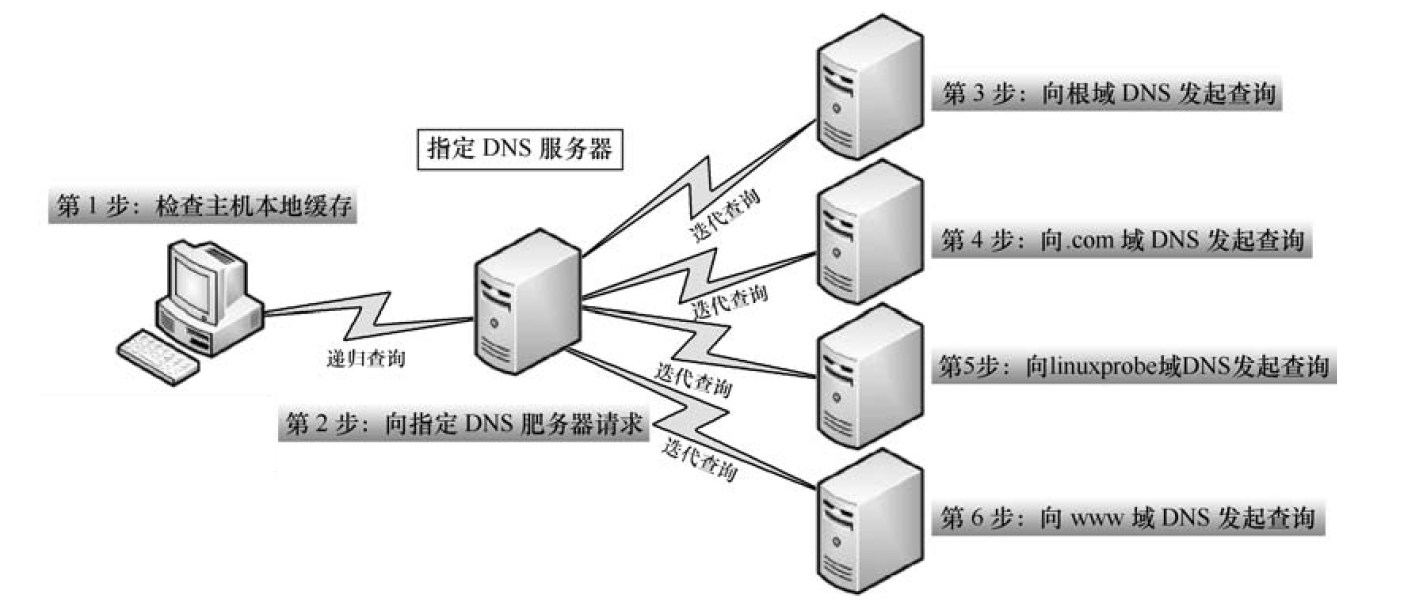
\includegraphics[width=0.8\linewidth]{image/DNS}
\end{figure}
当用户向网络指定的DNS 服务器发起一个域名请求时,通常情况下会有本地由此DNS
服务器向上级的DNS 服务器发送迭代查询请求;如果该DNS 服务器没有要查询的信息,则
会进一步向上级DNS 服务器发送迭代查询请求,直到获得准确的查询结果为止。

\begin{enumerate}
	\item 在浏览器中输入www.baidu.com域名,操作系统会先检查自己本地的hosts文件是否有这个网址映射关系,如果有,就先调用这个IP地址映射,完成域名解析。
	
	\item  如果hosts里没有这个域名的映射,则查找本地DNS解析器缓存,是否有这个网址映射关系,如果有,直接返回,完成域名解析。
	
	\item  如果hosts与本地DNS解析器缓存都没有相应的网址映射关系,首先会找TCP/ip参数中设置的首选DNS服务器(常见8.8.8.8;114.114.114.114)在此我们叫它本地DNS服务器,此服务器收到查询时,如果要查询的域名,包含在本地配置区域资源中,则返回解析结果给客户机,完成域名解析,此解析具有权威性。
	
	\item  如果本地DNS服务器本地区域文件与缓存解析都失效,则根据本地DNS服务器的设置(是否设置转发器)进行查询,如果未用转发模式,本地DNS就把请求发至13台根DNS,根DNS服务器收到请求后会判断这个域名(.com)是谁来授权管理,并会返回一个负责该顶级域名服务器的一个IP。本地DNS服务器收到IP信息后,将会联系负责.com域的这台服务器。这台负责.com域的服务器收到请求后,如果自己无法解析,它就会找一个管理.com域的下一级DNS服务器地址(baidu.com)给本地DNS服务器。当本地DNS服务器收到这个地址后,就会找baidu.com域服务器,重复上面的动作,进行查询,直至找到www.baidu.com主机。
	
	\item  如果用的是转发模式,此DNS服务器就会把请求转发至上一级DNS服务器,由上一级服务器进行解析,上一级服务器如果不能解析,或找根DNS或把转请求转至上上级,以此循环。不管是本地DNS服务器用是是转发,还是根提示,最后都是把结果返回给本地DNS服务器,由此DNS服务器再返回给客户机。
\end{enumerate}
\subsection{查看域名解析关系}
我们可以通过ns lookup命令查看域名的解析关系,但是该命令需要单独安装.
\hdrule{查看域名解析关系}
	\begin{ascboxB}{1.安装DNS服务套件:}
\begin{minted}{vim}
|\color{purple!80}{[root@localhost ~]#}| yum install bind-utils -y
Loaded plugins: fastestmirror
Loading mirror speeds from cached hostfile
.......
\end{minted}
	\end{ascboxB}
	\begin{ascboxB}{2.使用nslookup命令,nameserver lookup域名服务查找:}
\begin{minted}{vim}
|\color{purple!80}{[root@localhost ~]#}| nslookup azurekite.cn
Server:     119.29.29.29
Address:    119.29.29.29#53

Non-authoritative answer:
Name:    azurekite.cn
Address: 101.201.210.251
\end{minted}
	\end{ascboxB}
也可以通过交互式进行查询
\begin{enumerate}
\item 从主机名查询IP的流程称为:\md{正解}
\item 从IP反解析到主机名的流程称为:\md{反解}
\item 不管是正解还是反解,每个域的记录就是一个Zone, 例如把上述查到的记录称为数据库,而在数据库里面针对每个要解析的域(domaim),称为一个区域
\end{enumerate}
	\begin{ascboxB}{3.通过ping命令进行查找:}
\begin{minted}{vim}
|\color{purple!80}{[root@localhost ~]#}| ping azurekite.cn
PING azurekite.cn (101.201.210.251) 56(84) bytes of data.
64 bytes from 101.201.210.251 (101.201.210.251): icmp_seq=1 ttl=128 time=27.4 ms
64 bytes from 101.201.210.251 (101.201.210.251): icmp_seq=2 ttl=128 time=27.6 ms
64 bytes from 101.201.210.251 (101.201.210.251): icmp_seq=3 ttl=128 time=28.5 ms
64 bytes from 101.201.210.251 (101.201.210.251): icmp_seq=4 ttl=128 time=30.8 ms
\end{minted}
	\end{ascboxB}
\btrule{}

\subsection{linux的DNS配置文件}
接下来,我们看一下在Linux当中的关于DNS相关的配置文件.这里暂时有两个,分别是
\mintinline{shell}{/etc/host}和 \mintinline{shell}{/etc/resolv.conf}
\begin{enumerate}
\item \mintinline{shell}{/etc/host}: 该文件是运维人员自由定义域名和IP强制解析关系的
\item \mintinline{shell}{/etc/resolv.conf}: 该文件是,填入的是互联网中DNS服务器地址
\end{enumerate}
\hdrule{DNS解析测试2}
\begin{ascboxB}{1.\mintinline{shell}{/etc/host}文件修改:}
\begin{minted}{vim}
|\color{purple!80}{[root@localhost ~]#}| vim /etc/hosts
127.0.0.1   localhost localhost.localdomain localhost4 localhost4.localdomain4
::1         localhost localhost.localdomain localhost6 localhost6.localdomain6
127.0.0.1 azurekite.cn

|\color{purple!80}{[root@localhost ~]#}| ping azurekite.cn
PING azurekite.cn (127.0.0.1) 56(84) bytes of data.
64 bytes from localhost (127.0.0.1): icmp_seq=1 ttl=64 time=0.079 ms
64 bytes from localhost (127.0.0.1): icmp_seq=2 ttl=64 time=0.035 ms
64 bytes from localhost (127.0.0.1): icmp_seq=3 ttl=64 time=0.039 ms
\end{minted}
当我们修改\mintinline{shell}{/etc/host}文件之后,原本解析azurekite.cn的网站IP变为127.0.0.1我们设置的本地回环地址. 测试完成之后,再将该内容删除.
	\end{ascboxB}
	\begin{ascboxB}{2. \mintinline{shell}{/etc/resolv.conf}文件修改:}
\begin{minted}[
firstnumber=1,
highlightlines={5}]{vim}
|\color{purple!80}{[root@localhost ~]#}| vim /etc/resolv.conf
# Generated by NetworkManager
nameserver 119.29.29.29

# PS: 我们将/etc/resolv.conf文件中的内容删除
|\color{purple!80}{[root@localhost ~]#}| ping azurekite.cn
ping: azurekite.cn: Name or service not known
\end{minted}

这里我们发现azurekite.cn该网站已经无法通过域名进行访问了. 若我们将host文件进行第二次更改,则可以正常访问,因此需要注意的是,\mintinline{shell}{/etc/host}文件的解析优先级是要高于 \mintinline{shell}{/etc/resolv.conf}文件的。
	\end{ascboxB}
\btrule{}

以上就是DNS客户端的配置,客户端正常配置可以保证用户正常访问互联网,那么服务端又是什么样子的呢,还有DNS劫持是个什么玩意!

如果是小型 的域名解析需求,使用dnsmasq即可.大型的则可使用安装bind服务 
\section{DNS服务搭建之dnsmasq}
\begin{enumerate}
\item dnsmasq是一款小巧且方便地用于配置DNS服务器和DHCP服务器的工具,适用于小型网络,它提供了DNS解析功能和可选择的DHCP功能。 
\item dnsmasq可以解决小范围的dns查询问题,如果业务是跨机房、跨地区的话不建议使用dnsmasq做为dns解析服务器。
\end{enumerate}

\hdrule{dnsmasq的基本使用}
\begin{ascboxB}{1.  dnsmasq服务安装:}
\begin{minted}{vim}
|\color{purple!80}{[root@localhost ~]#}| yum install dnsmasq -y
Loaded plugins: fastestmirror
Loading mirror speeds from cached hostfile
\end{minted}
\end{ascboxB}
	\begin{ascboxB}{2.主配置文件,安装后自动生成:}
\begin{minted}{vim}
|\color{purple!80}{[root@localhost mail]#}| grep -Ev '^$|^[#;]' /etc/dnsmasq.conf
conf-dir=/etc/dnsmasq.d,.rpmnew,.rpmsave,.rpmorig
\end{minted}
\end{ascboxB}
	\begin{ascboxB}{3. 修改dnsmasq.conf,大概如下参数}
\begin{minted}[
highlightcolor=orange!10,
firstnumber=1,
highlightlines={1,4,8,12,15,18,21}]{vim}
# 指定上游dns服务器参数
resolv-file=/etc/resolv.dnsmasq.conf

# 访问baidu.com时的所有域名都会被解析成101.201.210.251
address=/baidu.com/101.201.210.251
address=/taobao.com/101.201.210.251

# 定义dnsmasq监听的地址,默认是监控本机的所有网卡上。局域网内主机若要使用dnsmasq服务时, 指定本机的IP地址
listen-address=192.168.178.180

#本地域名配置文件(不支持泛域名),添加内部需要解析的地址和域名(重新加载即可生效)
addn-hosts=/etc/dnsmasq.hosts  #  这个要写进去

#记录dns查询日志服务器
log-queries

# 设置日志记录
log-facility=/var/log/dnsmasq.log

#包含其他文件夹下所有配置文件
conf-dir=/etc/dnsmasq.d,.rpmnew,.rpmsave,.rpmorig
\end{minted}
	\end{ascboxB}
	\begin{ascboxB}{4.查看修改后的配置文件:}
\begin{minted}{vim}
|\color{purple!80}{[root@localhost ~]#}| grep -Ev '^$|^#' /etc/dnsmasq.conf
resolv-file=/etc/resolv.dnsmasq.conf
address=/baidu.com/101/201.210.251
address=/taobao.com/101/201/210.251
listen-address=192.168.178.220
addn-hosts=/etc/dnsmasq.hosts
log-queries
conf-dir=/etc/dnsmasq.d
conf-dir=/etc/dnsmasq.d,.bak
conf-dir=/etc/dnsmasq.d/,*.conf
conf-dir=/etc/dnsmasq.d,.rpmnew,.rpmsave,.rpmorig
\end{minted}
\end{ascboxB}
\btrule{}

上面我们修改了dnsmasq的主要配置文件,下面我们开始修改dnsmasq其他配置文件.

\hdrule{dnsmasq相关配置文件修改}
\begin{ascboxB}{1. 内部需要解析的ip和域名}
dnsmasp内部解析所需要的ip和域名,也就是用户所需要自定义的域名和ip的对应关系

\begin{minted}{vim}
[root@localhost /]# cat /etc/dnsmasq.hosts  # 注意该文件需要手动创建
101.201.210.251 azurekite.cn
\end{minted}
	\end{ascboxB}
\begin{ascboxB}{2.dnsmasq的上游DNS服务器}
\begin{minted}[highlightcolor=orange!10,firstnumber=1,highlightlines={1}]{vim}
#  /etc/resolv.dnsmasq.conf # 注意该文件需要手动创建 # 可以配置为resolv.conf,添加nameserver

[root@localhost /]# cat /etc/resolv.dnsmasq.conf
nameserver 119.29.29.29
nameserver 223.5.5.5
\end{minted}
\end{ascboxB}

\begin{ascboxB}{3. 启动dnsmasq服务}
\begin{minted}{vim}
|\color{purple!80}{[root@localhost ~]#}| systemctl start dnsmasq
|\color{purple!80}{[root@localhost ~]#}| systemctl status dnsmasq
|{$\bullet$}| dnsmasq.service - DNS caching server.
   Loaded: loaded (/usr/lib/systemd/system/dnsmasq.service; disabled; vendor preset: disabled)
   Active: active |\color{green}{\textbf{(running)}}| since Thu 2021-11-11 20:05:22 CST; 3s ago
 Main PID: 17202 (dnsmasq)
   CGroup: /system.slice/dnsmasq.service
        └──17202 /usr/sbin/dnsmasq -k

Nov 11 20:05:22 localhost.localdomain systemd[1]: Started DNS caching server..
Nov 11 20:05:22 localhost.localdomain dnsmasq[17202]: using nameserver 223.5.5.5#53
Nov 11 20:05:22 localhost.localdomain dnsmasq[17202]: read /etc/hosts - 2 addresses
Hint: Some lines were ellipsized, use -l to show in full.
\end{minted}
\end{ascboxB}

\begin{ascboxB}{4. 配置dns客户端地址}
正常来说,我们访问百度地址应该是我们预定义好的地址,但是实际并没有.
\begin{minted}[highlightcolor=orange!10,
breakanywhere,firstnumber=1,highlightlines={1}]{vim}
# 此时我们本地机器,还是用的本地预定义的dns的/etc/resolv.conf,对此进行修改
|\color{purple!80}{[root@localhost ~]#}| cat /etc/resolv.conf
# Generated by NetworkManager
# nameserver 119.29.29.29  # 使用定义的dnsmasq地址
nameserver 192.168.178.220
\end{minted}
\end{ascboxB}

\begin{ascboxB}{5. 测试dns域名解析}
\begin{minted}[highlightcolor=orange!10,firstnumber=1,highlightlines={1,9,15,22,}]{vim}
|\color{purple!80}{[root@localhost ~]#}| nslookup
> azurekite.cn
Server:         192.168.178.220     # 使用的是本地服务器
Address:        192.168.178.220#53

Non-authoritative answer:
Name:   azurekite.cn
Address: 101.201.210.251
> azurekitess.cn   # 预定义的假域名也可以解析到指定的IP上
Server:         192.168.178.220
Address:        192.168.178.220#53

Name:   azurekitess.cn
Address: 101.201.210.251
> baidu.com     # 百度的域名也可以解析到指定IP上
Server:         192.168.178.220
Address:        192.168.178.220#53

Name:   baidu.com
Address: 101.201.210.251

|\color{purple!80}{[root@localhost ~]#}| nslookup www.jd.com  # 京东的域名,则可以通过上游服务器进行解析
Server:         192.168.178.220
Address:        192.168.178.220#53
Non-authoritative answer:
www.jd.com      canonical name = www.jd.com.gslb.qianxun.com.
www.jd.com.gslb.qianxun.com     canonical name = cloud.jdcdn.com.
cloud.jdcdn.com canonical name = 11.jd.cdn.dnsv1.com.
11.jd.cdn.dnsv1.com     canonical name = 1036149.sched.skalego-dk.tdnsv5.com.
Name:   1036149.sched.skalego-dk.tdnsv5.com
Address: 113.137.62.49
\end{minted}
\end{ascboxB}
\btrule{}

以上就是dnsmasq,它可以解决小范围的dns查询问题,但是如果涉及到的业务是跨机房、跨地区的话,则使用另一个DNS服务,bind服务.

\section{DNS服务搭建之BIND}
BIND(Berkeley Internet Name Domain,伯克利因特网名称域)服务是全球范围内使用最广泛、最安全可靠且高效的域名解析服务程序。DNS 域名解析服务作为互联网基础设施服务,其责任之重可想而知,因此建议大家在生产环境中安装部署bind 服务程序时加上chroot(俗称牢笼机制)扩展包,以便有效地限制bind 服务程序仅能对自身的配置文件进行操作,以确保整个服务器的安全。

\hdrule{BIND服务的基本知识}
\begin{ascboxB}{1.  bind服务安装:}
\begin{minted}{vim}
|\color{purple!80}{[root@localhost ~]#}| um install bind-chroot
Loaded plugins: fastestmirror
Determining fastest mirrors
 * base: mirrors.163.com
 * extras: mirrors.163.com
 * updates: mirrors.huaweicloud.com
\end{minted}
\end{ascboxB}

bind 服务程序的配置并不简单,因为要想为用户提供健全的DNS 查询服务,要在本地保存相关的域名数据库,而如果把所有域名和IP 地址的对应关系都写入到某个配置文件中,估计要有上千万条的参数,这样既不利于程序的执行效率,也不方便日后的修改和维护。因此在bind 服务程序中有下面这三个比较关键的文件。
\begin{enumerate}
\item 主配置文件 \mintinline{shell}{/etc/named.conf}:只有58 行,而且在去除注释信息和空行之后,实际有效的参数仅有30 行左右,这些参数用来定义bind 服务程序的运行。
\item 区域配置文件\mintinline{shell}{/etc/named.rfc1912.zones}:用来保存域名和IP 地址对应关系的所在位置。类似于图书的目录,对应着每个域和相应IP 地址所在的具体位置,当需要查看或修改时,可根据这个位置找到相关文件。
\item 数据配置文件目录\mintinline{shell}{/var/named}:该目录用来保存域名和IP 地址真实对应关系的数据配置文件。
\end{enumerate}
\btrule{}
\subsection{DNS案例}
某校园网要架设一台 DNS 服务器来负责 long.com 域的域名解析工作。DNS 服务器的 FQDN 为 dns.long.com, IP 地址为 192.168.178.1。要求为以下域名实现正反向域名解析服务。

\[
\begin{array}{lll}
\text { dns.long.com }&~& 192.168 .178.1 \\
\text { mail.long.com }& ~& 192.168 .178 .2 \\
\text { slave.long.com } &\xleftrightarrow{\quad\text{MX记录}\quad} & 192.168.178.3 \\
\text { www.long.com }& ~& 192.168 .178.4 \\
\text { ftp.long.com }& ~& 192.168 .178.20
\end{array}
\]

另外, 为 www. long. com 设置别名为 web. long. com。
\hdrule{配置过程}
配置过程包括全局配置文件、主配置文件和正反向区域解析文件的配置。
\begin{ascboxB}{1.  编辑全局配置文件\mintinline{shell}{/etc/named.conf}}
\begin{minted}{vim}
|\color{purple!80}{[root@localhost ~]#}| vim /etc/named.conf
options {
        listen-on port 53 { any; };             # 修改
        listen-on-v6 port 53 { ::1; };
        directory       "/var/named";
        dump-file       "/var/named/data/cache_dump.db";
        statistics-file "/var/named/data/named_stats.txt";
        memstatistics-file "/var/named/data/named_mem_stats.txt";
        recursing-file  "/var/named/data/named.recursing";
        secroots-file   "/var/named/data/named.secroots";
        allow-query     { any; };               # 修改
        recursion yes;
        dnssec-enable yes;
        dnssec-validation no;           # 改为no可以忽略SELinux的影响

        bindkeys-file "/etc/named.root.key";
        managed-keys-directory "/var/named/dynamic";
        pid-file "/run/named/named.pid";    # 上面我们复制了,所以这里使用这个进行配置
        session-keyfile "/run/named/session.key";
};

logging {
        channel default_debug {
                file "data/named.run";
                severity dynamic;
        };
};

zone "." IN {
        type hint;
        file "named.ca";
};

include "/etc/named.zones";
include "/etc/named.root.key";
\end{minted}
\end{ascboxB}
\begin{ascboxB}{2.  配置主配置文件\mintinline{shell}{named.zones}}
\quad 该文件最后增加如下内容:
\begin{minted}{vim}
|\color{purple!80}{[root@localhost ~]#}| cp -p /etc/named.rfc1912.zones /etc/named.zones
|\color{purple!80}{[root@localhost ~]#}| vim /etc/named.zones
zone "long.com" IN {
        type master;
        file "long.com.zone";
        allow-update { none; };
};
zone "178.168.192.in-addr.arpa" IN {
        type master;
        file "1.178.168.192.zone";
        allow-update { none; };
};
\end{minted}
\end{ascboxB}
\begin{ascboxB}{2.  修改 BIND的区域配置文件}
\quad \md{第一步创建 long.com.zone 正向区域文件}
\begin{minted}{vim}
|\color{purple!80}{[root@localhost ~]#}| cp -p /var/named/named.localhost /var/named/long.com.zone
|\color{purple!80}{[root@localhost ~]#}| vim /var/named/long.com.zone
$TTL 1D
@       IN SOA  @ rname.invalid. (
                                        0       ; serial
                                        1D      ; refresh
                                        1H      ; retry
                                        1W      ; expire
                                        3H )    ; minimum

@     IN NS       dns.long.com.
@     IN MX  10  mail.long.com.

dns IN A 192.168.178.1
mail IN A 192.168.178.2
slave IN A 192.168.178.3
www IN A 192.168.178.4
ftp IN A 192.168.178.20
web IN CNAME www.long.com
\end{minted}
\quad \md{第二步创建1.178.168.192. zone反向区域文件}
\begin{minted}{vim}
|\color{purple!80}{[root@localhost ~]#}| cp -p /var/named/named.loopback /var/named/1.178.168.192.zone
|\color{purple!80}{[root@localhost ~]#}| vim /var/named/1.178.168.192.zone
$TTL 1D
@       IN SOA  @ rname.invalid. (
                                        0       ; serial
                                        1D      ; refresh
                                        1H      ; retry
                                        1W      ; expire
                                        3H )    ; minimum

@   IN  NS      dns.long.com.
@   IN  MX  10  mail.long.com.

1     IN PTR  dns.long.com.
2    IN PTR  mail.long.com.
3    IN PTR  slave.long.com.
4    IN PTR  www.long.com.
20  IN PTR  ftp.long.com.
\end{minted}
\end{ascboxB}
\begin{ascboxB}{3. 设置防火墙放行}
\begin{minted}{vim}
|\color{purple!80}{[root@localhost ~]#}| firewall-cmd --permanent --add-service=dns 
success
|\color{purple!80}{[root@localhost ~]#}| firewall-cmd --reload
success
\end{minted}
\end{ascboxB}
\begin{ascboxB}{4. 检查配置文件是否有错误}
\begin{minted}{vim}
|\color{purple!80}{[root@localhost ~]#}| named-checkconf /etc/named.conf
|\color{purple!80}{[root@localhost ~]#}| named-checkzone 178.168.192.in-addr.arpa /var/named/1.178.168.192.zone
zone 178.168.192.in-addr.arpa/IN: 178.168.192.in-addr.arpa/MX 'mail.long.com' (out of zone) has no addresses records (A or AAAA)
zone 178.168.192.in-addr.arpa/IN: loaded serial 0
OK
\end{minted}
\end{ascboxB}

\begin{ascboxB}{5. 重新启动 DNS 服务,检查运行状态}
\begin{minted}{vim}
|\color{purple!80}{[root@localhost ~]#}| systemctl start named
|\color{purple!80}{[root@localhost ~]#}| systemctl status named
|{$\bullet$}| named.service - Berkeley Internet Name Domain (DNS)
   Loaded: loaded (/usr/lib/systemd/system/named.service; disabled; vendor preset: disabled)
   Active: |\color{green!80}{active (running)}| since Wed 2021-11-24 14:42:52 CST; 1s ago
  Process: 7940 ExecStart=/usr/sbin/named -u named -c ${NAMEDCONF} $OPTIONS (code=exited, status=0/SUCCESS)
  Process: 7937 ExecStartPre=/bin/bash -c if [ ! "$DISABLE_ZONE_CHECKING" == "yes" ]; then /usr/sbin/named-checkconf -z "$NAMEDCONF"; else echo "Checking of zone files is disabled";  
  fi (code=exited, status=0/SUCCESS)
 Main PID: 7942 (named)
   CGroup: /system.slice/named.service
       └──7942 /usr/sbin/named -u named -c /etc/named.conf

.....................................
Nov 24 14:42:53 localhost.localdomain named[7942]: managed-keys-zone: Key 20326 for zone . acceptance timer complete: key...usted
Nov 24 14:42:53 localhost.localdomain named[7942]: resolver priming query complete
Hint: Some lines were ellipsized, use -l to show in full.
\end{minted}
\end{ascboxB}

\begin{ascboxB}{6. 配置客户端}
\begin{minted}{vim}
|\color{purple!80}{[root@localhost ~]#}| vim /etc/resolv.conf
# Generated by NetworkManager
nameserver 119.29.29.29
nameserver 192.168.178.220
nameserver 192.168.178.1
nameserver 192.168.178.2
search long.com
\end{minted}
\end{ascboxB}
\btrule{}

\section{ssh服务和SSHD服务环境}
SSH(Secure Shell)是一种能够以安全的方式提供远程登录的协议,也是目前远程管理Linux 系统的首选方式。在此之前,一般使用FTP 或Telnet 来进行远程登录。但是因为它们以明文的形式在网络中传输账户密码和数据信息,因此很不安全,很容易受到黑客发起的中间人攻击,这轻则篡改传输的数据信息,重则直接抓取服务器的账户密码。想要使用 SSH 协议来远程管理Linux 系统,则需要部署配置sshd 服务程序。sshd 是基于SSH协议开发的一款远程管理服务程序,不仅使用起来方便快捷,而且能够提供两种安全验证的方法:
\begin{itemize}
\item 基于口令的验证—用账户和密码来验证登录;对称加密(秘钥加密)
\item 基于密钥的验证—需要在本地生成密钥对,然后把密钥对中的公钥上传至服务器,并与服务器中的公钥进行比较;该方式相较来说更安全。非对称加密(公钥加密)
\end{itemize}

\subsection{ssh免密登录}
\hdrule{配置过程}
配置过程包括全局配置文件、主配置文件和正反向区域解析文件的配置。
\begin{ascboxB}{ssh免密登录配置实战}
\begin{minted}{vim}
# 第一步: 客户端本地生成一对公私钥
ssh-keygen -t rsa  #  该命令输入后,默认回车即可

# 第二步: 客户端发送自己的公钥, 发给服务器, 存在服务器的authorized_keys文件中
ssh-copy-id root@192.168.178.110

# 第三步: 此时直接输入登录命令, 即可免密登录了
ssh root@192.168.178.110

# 第四步: 登录服务器, 检查客户端的公钥信息
[root@localhost ~]# cat ~/.ssh/authorized_keys
ssh-rsa AAAAB3NzaC1yc2EAAAADAQABAAABgQDN2JBaA6w/k1CNZQXoXYKvnkHC1wrvSuVl5Hj/YxetQzRXt4yGKa/e9fX4glQvcoJ/SVHX7klXYGrDGBPEMYFjU+hKFLNhieIjXJg8Yc6mUJ9OlUL4E3di25mAFSyu0l2XSDxLw2zgoZ.........
\end{minted}
\end{ascboxB}
\btrule{}

\subsection{SSHD服务详细配置}
基本上,所有的 sshd 服务器详细设定都放在 \texttt{/etc/ssh/sshd\_config} 里面!不过,每个 Linux distribution 的预设设定都不太相同,所以我们有必要来了解一下整个设定值的意义!
\hdrule{SSHD配置文件详解}
\begin{ascboxB}{\mintinline{shell}{/etc/ssh/sshd_config}配置文件详解}
\begin{minted}{vim}
#    $OpenBSD: sshd_config,v 1.100 2016/08/15 12:32:04 naddy Exp $

# This is the sshd server system-wide configuration file.  See
# sshd_config(5) for more information.

# This sshd was compiled with PATH=/usr/local/bin:/usr/bin

# The strategy used for options in the default sshd_config shipped with
# OpenSSH is to specify options with their default value where
# possible, but leave them commented.  Uncommented options override the
# default value.

# If you want to change the port on a SELinux system, you have to tell
# SELinux about this change.
# semanage port -a -t ssh_port_t -p tcp #PORTNUMBER
#
#Port 22                # 默认端口
#AddressFamily any      # 配置地址家族,any支持ipv4,ipv6
#ListenAddress 0.0.0.0  # 设置sshd服务监听的ip地址,注意多网卡的绑定
#ListenAddress ::

# ssh各密钥存放的位置
HostKey /etc/ssh/ssh_host_rsa_key       # SSH version 2 使用的RSA私钥
#HostKey /etc/ssh/ssh_host_dsa_key      # SSH version 2 使用的DSA私钥
HostKey /etc/ssh/ssh_host_ecdsa_key     
HostKey /etc/ssh/ssh_host_ed25519_key

# Ciphers and keying
#RekeyLimit default none

# Logging
#SyslogFacility AUTH
SyslogFacility AUTHPRIV
#LogLevel INFO              # 登录记录的等级

# Authentication:           # 登入设定部分

#LoginGraceTime 2m          # 当使用者连上SSH server之后,会出现输入密码的画面,在该画面中在多久时间内没有成功连上SSH server就强迫断线!若无单位则默认时间为秒
#PermitRootLogin yes        # 是否允许root管理员直接登录,保证系统安全
#StrictModes yes            # 当用户的私钥改变,直接拒绝连接
#MaxAuthTries 6             # 最大密码尝试次数
#MaxSessions 10             # 最大终端数

#PubkeyAuthentication yes   # 是否允许用户自行使用成对的密钥系统进行登入行为,仅针对version2。

# The default is to check both .ssh/authorized_keys and .ssh/authorized_keys2
# but this is overridden so installations will only check .ssh/authorized_keys
AuthorizedKeysFile    .ssh/authorized_keys      # 信任主机的公钥文件存放地

#AuthorizedPrincipalsFile none

#AuthorizedKeysCommand none
#AuthorizedKeysCommandUser nobody

# For this to work you will also need host keys in /etc/ssh/ssh_known_hosts
#HostbasedAuthentication no
# Change to yes if you don't trust ~/.ssh/known_hosts for
# HostbasedAuthentication
#IgnoreUserKnownHosts no
# Don't read the user's ~/.rhosts and ~/.shosts files
#IgnoreRhosts yes

# To disable tunneled clear text passwords, change to no here!
#PasswordAuthentication yes     
#PermitEmptyPasswords no        # 是否允许空密码登录,禁止
PasswordAuthentication yes      # 是否设置密码验证机制

# Change to no to disable s/key passwords
#ChallengeResponseAuthentication yes        # 允许任何的密码认证!所以,任何 login.conf 规定的认证方式,均可适用
ChallengeResponseAuthentication no          # 但目前我们比较喜欢使用 PAM 模块帮忙管理认证,因此这个选项可以设定为 no

# Kerberos options              # 与Kerberos有关的参数设定!因为我们没有Kerberos主机,所以底下不用设定
#KerberosAuthentication no
#KerberosOrLocalPasswd yes
#KerberosTicketCleanup yes
#KerberosGetAFSToken no
#KerberosUseKuserok yes

# GSSAPI options
GSSAPIAuthentication yes
GSSAPICleanupCredentials no
#GSSAPIStrictAcceptorCheck yes
#GSSAPIKeyExchange no
#GSSAPIEnablek5users no

# Set this to 'yes' to enable PAM authentication, account processing,
# and session processing. If this is enabled, PAM authentication will
# be allowed through the ChallengeResponseAuthentication and
# PasswordAuthentication.  Depending on your PAM configuration,
# PAM authentication via ChallengeResponseAuthentication may bypass
# the setting of "PermitRootLogin without-password".
# If you just want the PAM account and session checks to run without
# PAM authentication, then enable this but set PasswordAuthentication
# and ChallengeResponseAuthentication to 'no'.
# WARNING: 'UsePAM no' is not supported in Red Hat Enterprise Linux and may cause several
# problems.
UsePAM yes                  # 利用 PAM 管理使用者认证有很多好处,可以记录与管理。

#AllowAgentForwarding yes
#AllowTcpForwarding yes
#GatewayPorts no
X11Forwarding yes
#X11DisplayOffset 10
#X11UseLocalhost yes
#PermitTTY yes
#PrintMotd yes
#PrintLastLog yes           # 显示上次登入的信息
#TCPKeepAlive yes           # 当达成联机后,服务器会一直传送 TCP 封包给客户端藉以判断对方式否一直存在联机。
#UseLogin no
#UsePrivilegeSeparation sandbox
#PermitUserEnvironment no
#Compression delayed
#ClientAliveInterval 0
#ClientAliveCountMax 3
#ShowPatchLevel no
#UseDNS yes             # 一般来说,为了要判断客户端来源是正常合法的,因此会使用 DNS 去反查客户端的主机名不过如果是在内网互连,这项目设定为no会让联机达成速度比较快。
#PidFile /var/run/sshd.pid
#MaxStartups 10:30:100
#PermitTunnel no
#ChrootDirectory none
#VersionAddendum none

# no default banner path
#Banner none

# Accept locale-related environment variables
AcceptEnv LANG LC_CTYPE LC_NUMERIC LC_TIME LC_COLLATE LC_MONETARY LC_MESSAGES
AcceptEnv LC_PAPER LC_NAME LC_ADDRESS LC_TELEPHONE LC_MEASUREMENT
AcceptEnv LC_IDENTIFICATION LC_ALL LANGUAGE
AcceptEnv XMODIFIERS

# override default of no subsystems
Subsystem    sftp    /usr/libexec/openssh/sftp-server

# Example of overriding settings on a per-user basis
#Match User anoncvs
#    X11Forwarding no
#    AllowTcpForwarding no
#    PermitTTY no
#    ForceCommand cvs server
\end{minted}
\end{ascboxB}
\btrule{}











\end{document}
